%% Version 6.1, 1 September 2021

% This tex file can be compiled with
% tectonic templateV5.tex
% https://tectonic-typesetting.github.io
%
% Or simply with the Overleaf latexmkrc configuration: (included in the repo)
% https://www.overleaf.com/learn/how-to/How_does_Overleaf_compile_my_project%3F
%
% A latexindent.yml config file is also included for easier and more consistent
% formatting.

%%%%%%%%%%%%%%%%%%%%%%%%%%%%%%%%%%%%%%%%%%%%%%%%%%%%%%%%%%%%%%%%%%%%%%
% TemplateV6.1.tex --  LaTeX-based blank template for submissions to the
% American Meteorological Society
%
%%%%%%%%%%%%%%%%%%%%%%%%%%%%%%%%%%%%%%%%%%%%%%%%%%%%%%%%%%%%%%%%%%%%%
% PREAMBLE
%%%%%%%%%%%%%%%%%%%%%%%%%%%%%%%%%%%%%%%%%%%%%%%%%%%%%%%%%%%%%%%%%%%%%

%% Start with one of the following:
% 1.5-SPACED VERSION FOR SUBMISSION TO THE AMS
\documentclass{ametsocV6.1}

% TWO-COLUMN JOURNAL PAGE LAYOUT---FOR AUTHOR USE ONLY
% \documentclass[twocol]{ametsocV6.1}

%%%%%%%%%%%%%%%%%%%%%%%%%%%%%%
% FOR PRINTING
\usepackage[a4paper]{geometry}
% MY ADDITIONS
\usepackage{multirow}
\usepackage[separate-uncertainty=true]{siunitx}
\usepackage[version=4]{mhchem}
\usepackage[acronym]{glossaries}
\setacronymstyle{long-short}
\makeglossaries{}
\newacronym{agcm}{AGCM}{Atmosphere General Circulation Model}
\newacronym{aodm}{AODVISstdn}{``stratospheric aerosol optical depth 550 nm day night''}
\newacronym{aod}{AOD}{(stratospheric) aerosol optical depth}
\newacronym{aogcm}{AOGCM}{Atmosphere-Ocean General Circulation Model}
\newacronym{c2wmp}{C2W\(-\)}{CESM2(WACCM6) intermediate strength}
\newacronym{c2wm}{C2W\(\downarrow\)}{CESM2(WACCM6) small strength}
\newacronym{c2wsn}{C2WN\(\uparrow\)}{CESM2(WACCM6) large strength, high northern latitude}
\newacronym{c2ws}{C2W\(\uparrow\)}{CESM2(WACCM6) large strength}
\newacronym{c2w}{C2W}{CESM2(WACCM6) tropical}
\newacronym{cam5}{CAM5}{Community Atmosphere Model Version 5}
\newacronym{cam6}{CAM6}{Community Atmosphere Model Version 6}
\newacronym{cesm1}{CESM1}{Community Earth System Model Version 1}
\newacronym{cesm2}{CESM2}{Community Earth System Model Version 2}
\newacronym{cesm}{CESM}{Community Earth System Model}
\newacronym{cice}{CICE5}{CICE Version 5.1.2}
\newacronym{cime}{CIME}{Common Infrastructure for Modelling the Earth}
\newacronym{cism}{CISM2}{Community Ice Sheet Model Version 2.1}
\newacronym{clm}{CLM5}{Community Land Model Version 5}
\newacronym{ecs}{ECS}{equilibrium climate sensitivity}
\newacronym{erf}{ERF}{effective radiative forcing}
\newabbreviation{ob16}{OB16}{\citet{ottobliesner2016}}
\newacronym{esm}{ESM}{Earth System Model}
\newacronym{flnt}{FLNT}{``net longwave flux at the top of the model''}
\newacronym{fpp}{FPP}{Filtered Poisson Process}
\newacronym{fsnt}{FSNT}{``net solar flux at the top of the model''}
\newacronym{fsst}{\texttt{fSST1850}}{fixed sea-surface temperature}
\newacronym{irf}{IRF}{instantaneous radiative forcing}
\newacronym{lwcf}{LWCF}{``long wave cloud forcing''}
\newacronym{lw}{LW}{long wave}
\newacronym{mam3}{MAM3}{three mode version of the Modal Aerosol Module}
\newacronym{mam}{MAM}{Modal Aerosol Module}
\newacronym{marbl}{MARBL}{MARine Biogeochemistry Library}
\newacronym{ma}{MA}{middle atmosphere}
\newacronym{mosart}{MOSART}{MOdel for Scale Adaptive River Transport}
\newabbreviation{j05}{J05}{\citet{jones2005}}
\newabbreviation{g16}{G16}{\citet{gregory2016}}
\newabbreviation{m20}{M20}{\citet{marshall2020dataset}}
\newabbreviation{t10}{T10}{\citet{timmreck2010}}
\newabbreviation{n15}{N15}{\citet{niemeier2015}}
\newacronym{pop}{POP2}{Parallel Ocean Program Version 2}
\newacronym{qbo}{QBO}{quasi-biennial oscillation}
\newacronym{rf}{RF}{(effective) radiative forcing}
\newacronym{swcf}{SWCF}{``short wave cloud forcing''}
\newacronym{sw}{SW}{short wave}
\newacronym{tcrp}{TCRP}{transient climate response parameter}
\newacronym{toa}{TOA}{top-of-the-atmosphere}
\newacronym{trefht}{TREFHT}{``reference height temperature''}
\newacronym{waccm}{WACCM6}{Whole Atmosphere Community Climate Model Version 6}
\newacronym{ww3}{WW3}{Wave Watch Version 3}
\newacronym{ytt}{YTT}{Young Toba Tuff}

% Create some custom commands
\newcommand{\iso}[1][i]{{#1}njected \ce{SO2}}
% The content of the URL must be on its own line. The compiler works fine both ways, but
% the syntax highlighting is messed up by it.
\urldef\fssturl\url{
1850_CAM60%WCCM_CLM50%BGC-CROP_CICE%PRES_DOCN%DOM_MOSART_CISM2%NOEVOLVE_SWAV_TEST
}
%%%%%%%%%%%%%%%%%%%%%%%%%%%%%%

%%%%%%%%%%%%%%%%%%%%%%%%%%%%%%%%

%%% To be entered by author:

%% May use \\ to break lines in title:

\title{
  Parameter Scan: Volcanic influence on climate across multiple magnitudes of injected
  \ce{SO2}
}

%% Enter authors' names and affiliations as you see in the examples below.
%
%% Use \correspondingauthor{} and \thanks{} (\thanks command to be used for affiliations footnotes,
%% such as current affiliation, additional affiliation, deceased, co-first authors, etc.)
%% immediately following the appropriate author.
%
%% Note that the \correspondingauthor{} command is NECESSARY.
%% The \thanks{} commands are OPTIONAL.
%
%% Enter affiliations within the \affiliation{} field. Use \aff{#} to indicate the affiliation letter at both the
%% affiliation and at each author's name. Use \\ to insert line breaks to place each affiliation on its own line.

%\authors{Author One,\aff{a}\correspondingauthor{Author One, email@email.com}
%Author Two,\aff{a}
%Author Three,\aff{b}
%Author Four,\aff{a}
%Author Five\thanks{Author Five's current affiliation: NCAR, Boulder, Colorado},\aff{c}
%Author Six,\aff{c}
%Author Seven,\aff{d}
% and Author Eight\aff{a,d}
%}
%
%\affiliation{\aff{a}{First Affiliation}\\
%\aff{b}{Second Affiliation}\\
%\aff{c}{Third Affiliation}\\
%\aff{d}{Fourth Affiliation}
%}

\authors{
  Eirik Rolland Enger,\aff{a}\correspondingauthor{Eirik Rolland Enger, eirik.r.enger@uit.no}
  Rune Graversen,\aff{a}
  Martin Rypdal,\aff{a}
  Audun Theodorsen,\aff{a}
  and Maria Rugenstein\aff{b}
}

\affiliation{
  \aff{a}{UiT The Arctic University of Norway, Tromsø, Norway}\\
  \aff{b}{Colorado State University, Fort Collins, Colorado}
}

%%%%%%%%%%%%%%%%%%%%%%%%%%%%%%%%%%%%%%%%%%%%%%%%%%%%%%%%%%%%%%%%%%%%%
% ABSTRACT
%
% Enter your abstract here
% Abstracts should not exceed 250 words in length!
%

\abstract{%
  Large to super-volcano sized eruptions are simulated in the \glsentrylong{cesm2}
  (\glsentryshort{cesm2}) climate model with the \glsentrylong{waccm}
  (\glsentryshort{waccm}) atmosphere. Ensembles containing four members are simulated
  and the \glsentrylong{aod} (\glsentryshort{aod}) and \glsentrylong{rf}
  (\glsentryshort{rf}) from the eruptions are compared to determine how far the linear
  relationship between the two parameters hold. Simulating a Pinatubo-like eruption
  yields results consistent with several previous studies showing a slope of \(\sim
  \SI{-20}{\watt\metre^{-2}}\) per unit \glsentryshort{aod} for \glsentryshort{rf}.
  Larger eruptions, however, show a more shallow slope indicative of a lower cooling
  efficiency. Moreover, a time-after-eruption dependence between \glsentryshort{aod} and
  \glsentryshort{rf} is found, where the \glsentryshort{rf} is relatively stronger than
  \glsentryshort{aod} the first year after the eruption (higher cooling efficiency),
  while later their ratio is roughly constant for a given eruption strength.
}

\begin{document}

%% Necessary!
\maketitle

%%%%%%%%%%%%%%%%%%%%%%%%%%%%%%%%%%%%%%%%%%%%%%%%%%%%%%%%%%%%%%%%%%%%%
% SIGNIFICANCE STATEMENT/CAPSULE SUMMARY
%%%%%%%%%%%%%%%%%%%%%%%%%%%%%%%%%%%%%%%%%%%%%%%%%%%%%%%%%%%%%%%%%%%%%
%
% If you are including an optional significance statement for a journal article or a required capsule summary for BAMS
% (see www.ametsoc.org/ams/index.cfm/publications/authors/journal-and-bams-authors/formatting-and-manuscript-components for details),
% please apply the necessary command as shown below:
%
% Significance Statement (all journals except BAMS)
%
%\statement
%	 Enter significance statement here, no more than 120 words. See \url{www.ametsoc.org/index.cfm/ams/publications/author-information/significance-statements/} for details.
%
%% Capsule (BAMS only)
%%
%\capsule
%       Enter BAMS capsule here, no more than 30 words. See \url{www.ametsoc.org/index.cfm/ams/publications/author-information/formatting-and-manuscript-components/#capsule} for details.
%
%% * * If using twocol mode, you will need to use the commands "twocolsig" and "twocolcapsule" in place of "sig" and "capsule"
%%      to ensure that the text box correctly spans across both columns.
%

%%%%%%%%%%%%%%%%%%%%%%%%%%%%%%%%%%%%%%%%%%%%%%%%%%%%%%%%%%%%%%%%%%%%%
% MAIN BODY OF PAPER
%%%%%%%%%%%%%%%%%%%%%%%%%%%%%%%%%%%%%%%%%%%%%%%%%%%%%%%%%%%%%%%%%%%%%
%

%% In all cases, if there is only one entry of this type within
%% the higher level heading, use the star form:
%%
% \section{Section title}
% \subsection*{subsection}
% text...
% \section{Section title}

%vs

% \section{Section title}
% \subsection{subsection one}
% text...
% \subsection{subsection two}
% \section{Section title}

%%%
% \section{First primary heading}

% \subsection{First secondary heading}

% \subsubsection{First tertiary heading}

% \paragraph{First quaternary heading}

%%%%%%%%%%%%%%%%%%%%%%%%%%%%%%%%%%%%%%%%%%%%%%%%%%%%%%%%%%%%%%%%%%%%%
% TABLES---INSERT NEAR IN-TEXT DISCUSSION
%%%%%%%%%%%%%%%%%%%%%%%%%%%%%%%%%%%%%%%%%%%%%%%%%%%%%%%%%%%%%%%%%%%%%
%%  Enter tables near where they are discussed within the document.
%%  Please place tables before/after paragraphs, not within a paragraph.
%%
%
%\begin{table}[t]
%\caption{This is a sample table caption and table layout.  Enter as many tables as
%  necessary at the end of your manuscript. Table from Lorenz (1963).}\label{t1}
%\begin{center}
%\begin{tabular}{ccccrrcrc}
%\hline\hline
%$N$ & $X$ & $Y$ & $Z$\\
%\hline
% 0000 & 0000 & 0010 & 0000 \\
% 0005 & 0004 & 0012 & 0000 \\
% 0010 & 0009 & 0020 & 0000 \\
% 0015 & 0016 & 0036 & 0002 \\
% 0020 & 0030 & 0066 & 0007 \\
% 0025 & 0054 & 0115 & 0024 \\
%\hline
%\end{tabular}
%\end{center}
%\end{table}

%%%%%%%%%%%%%%%%%%%%%%%%%%%%%%%%%%%%%%%%%%%%%%%%%%%%%%%%%%%%%%%%%%%%%
% FIGURES---INSERT NEAR IN-TEXT DISCUSSION
%%%%%%%%%%%%%%%%%%%%%%%%%%%%%%%%%%%%%%%%%%%%%%%%%%%%%%%%%%%%%%%%%%%%%
%%  Enter figures near where they are discussed within the document.
%%  Please place figures before/after paragraphs, not within a paragraph.
% %
%
%\begin{figure}[t]
%  \noindent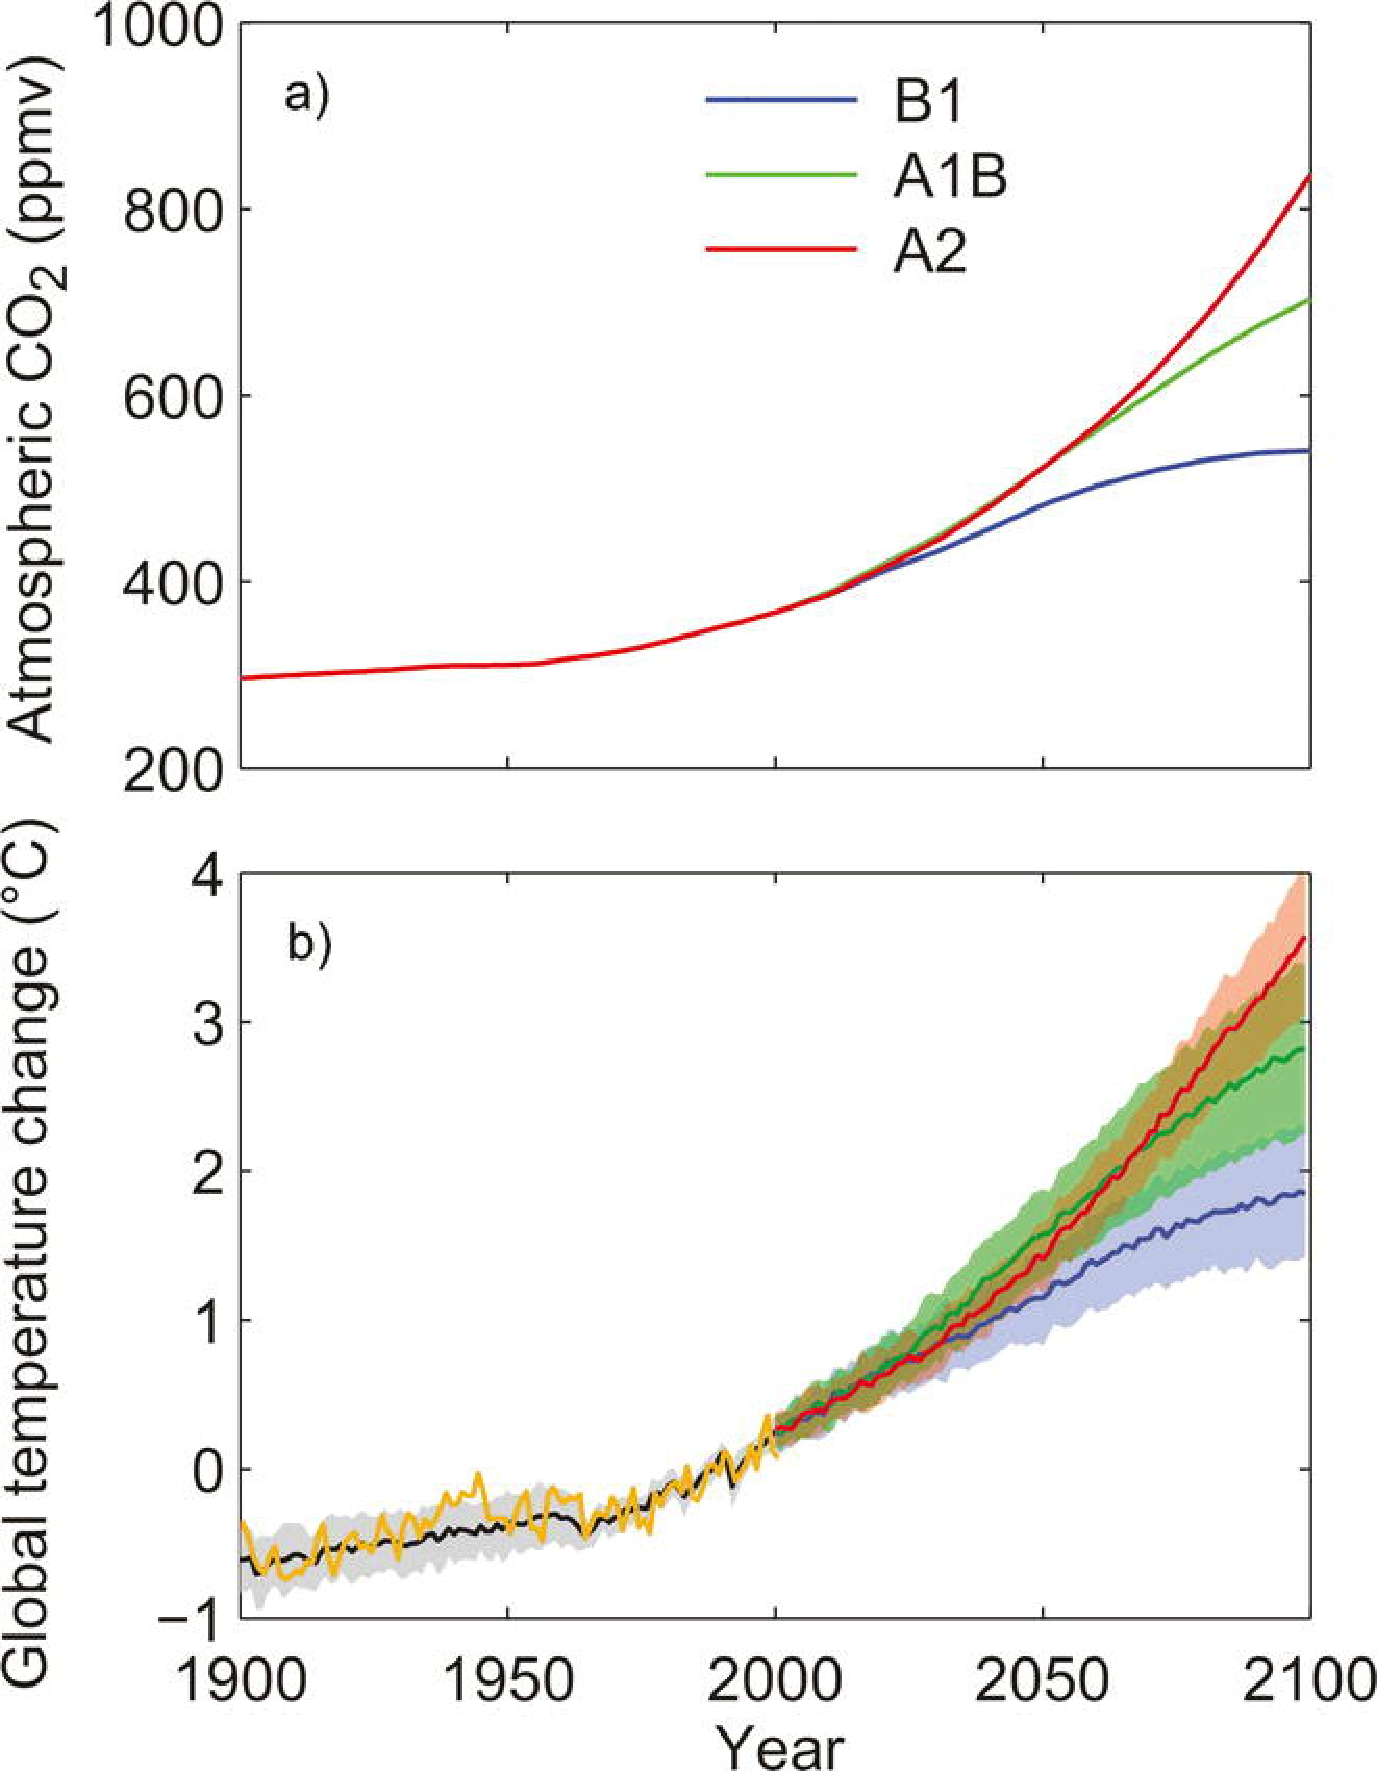
\includegraphics[width=19pc,angle=0]{figure01.pdf}\\
%  \caption{Enter the caption for your figure here.  Repeat as
%  necessary for each of your figures. Figure from \protect\cite{Knutti2008}.}\label{f1}
%\end{figure}

% NOTE: what to include in the paper, key questions.
% The paper should provide insight about what might happen if a large volcano erupted
% (order of magnitude or more than Mt.\ Pinatubo). How does the atmosphere react, for
% example in the aerosol dynamics? (QBO, SO2/AOD/RF relationship.) It should also be
% about how volcanic simulations compare in magnitude and if there is time for more
% simulations, how model complexity (dynamic ocean against slab ocean) affect things.
% - How far does the linear relation between AOD and RF go? What phases does the
%   aerosols go though? (Perhaps the most promising avenue.)
% - How much does it matter how high in the atmosphere the initial SO2 is injected?
%   (Already is some literature on this, suggesting it is not much. Also some on
%   latitude dependence, which has a bigger influence.)
% - How does the climate response change based on the state of the climate: what if we
%   run a CO2 doubling or quadrupling simulation until close to equilibrium, and let the
%   volcanoes erupt then? (Lack the doubling scenario, and setting it up has resulted in
%   strange output that must be resolved. Could take a while.)

\section{Introduction}

% NOTE: Suggested layout for the introduction
% - The objectives of the work.
% - The justification for these objectives: Why is the work important?
% - Background: Who else has done what? How? What have we done previously?
% - Guidance to the reader: What should the reader watch for in the paper? What are the
%   interesting high points? What strategy did we use?
% - Summary/conclusion: What should the reader expect as conclusion? In advanced
%   versions of the outline, you should also include all the sections that will go in
%   the Experimental section (at the level of paragraph subheadings) and indicate what
%   information will go.

% Toohey et al 2011 have a nice end of introduction.

The \gls{rf} and \gls{aod}, expressing the energy imbalance at \gls{toa} and the opacity
of the stratosphere due to aerosol scattering, are much used as measures to express the
forcing from large volcanic eruptions. Often the \gls{rf} is assumed to depend linearly
on the \gls{aod} \citep{myhre2013,andersson2015}, and several studies have shown such a
linear relationship to be good estimates when running climate model simulations of
volcanic eruptions \citep{mills2017,hansen2005,gregory2016,marshall2020,pitari2016b}.
Despite this, there is a wide spread in the estimated volcanic forcing efficiencies
among the studies, ranging between \(\sim \SI{15}{\watt\metre^{-2}\ce{AOD}^{-1}}\)
\citep{pitari2016b} and \(\sim \SI{25}{\watt\metre^{-2}\ce{AOD}^{-1}}\)
\citep{myhre2013}, with estimates being based on \gls{aod} values up to at most \(\sim
0.7\).

\ce{H2O}, \ce{N2} and \ce{CO2} are the most abundant gases emitted by volcanoes
\citep{robock2000}, but still, sulphur species like \ce{SO2} are the most influential
due to the already relatively high concentrations of the former gases in the atmosphere.
From \ce{SO2}, molecules of \ce{H2SO4} is formed after reactions with \ce{OH} and
\ce{H2O} \citep{robock2000}. Sulphate acid, \ce{H2SO4}, is backscattering sunlight and
hereby increasing the planetary albedo and thus the \gls{rf}. Since its formation from
\ce{SO2} is happening over weeks \citep{robock2000}, the peak \gls{rf} from the eruption
has a slight delay from the onset of the eruption. The duration of time that the
\ce{H2SO4} aerosols stay in the stratosphere depends on several factors, including
latitude \citep{marshall2019, toohey2019}, volcanic plume height \citep{marshall2019},
the aerosol size \citep{marshall2019}, the phase of the \gls{qbo} \citep{pitari2016b}
and the season of the year (determining to which hemisphere aerosols are transported)
\citep{toohey2011,toohey2019}. In the case of tropical eruptions, aerosols are typically
transported poleward in the stratosphere and back to mid-latitude troposphere within one
to two years \citep{robock2000}. As the aerosols eventually move below the tropopause
they are readily removed by wet deposition \citep{liu2012}.

Before the current strong anthropogenic forcing of the climate, during the Holocene
period, the climate variability on Earth was mostly forced by volcanic eruptions
\citep{sigl2022}. Despite the strong climate variability impact of volcanic eruptions,
few climate model experiments have included volcanic forcing when simulating climate
evolution during the Holocene \citep{sigl2022}, implying an exaggerated positive forcing
\citep{gregory2016,solomon2011}. This lack of a persistent cooling is one of several
factors that has been suggested to contribute to the discrepancy commonly found between
simulated and observed global warming \citep{andersson2015}. Even though the
understanding of how volcanic eruptions force the climate have been given much
attention, questions related to aerosol particle processes such as how they grow or the
rate at which they are created when \ce{OH} is not abundant are still unanswered
\citep[e.g.][]{robock2000,zanchettin2019,marshall2020,marshall2022}. These processes
impacts the aerosols scattering efficiency and possibly the \gls{rf} to \gls{aod}
relationship. \citet{marshall2020} present results showing higher efficiencies in years
2 and 3 after an eruption, compared to year 1, suggesting that this is due to the
aerosols being concentrated more spatially in the first year and more spread out in
later years. This has the effect of increasing the albedo per global mean \gls{aod}
which in turn increases the \gls{rf} to \gls{aod} ratio \citep{marshall2020}.

Previous studies on both Mt.\ Pinatubo alone \citep{mills2017,hansen2005} and volcanoes
in the instrumental era \citep{gregory2016} have been used to estimate the relationship
between the \gls{rf} energy imbalance and change in \gls{aod} caused by volcanic
eruptions. \citet{myhre2013} use a formula for \gls{rf} that scales \gls{aod} by
\(\SI{-25}{\watt\metre^{-2}\mathrm{AOD}^{-1}}\) while estimates down to
\(\SI{-19.0(5)}{\watt\metre^{-2}\mathrm{AOD}^{-1}}\) \citep{gregory2016} and
\(\SI{-18.3(10)}{\watt\metre^{-2}\mathrm{AOD}^{-1}}\) \citep{mills2017} have been
reported more recently. Simulations done with synthetic volcanoes have also been used,
and in \citet{marshall2020} they obtain a scaling factor of
\(\SI{-20.5(2)}{\watt\metre^{-2}\mathrm{AOD}^{-1}}\) from \(82\) simulations of volcanic
eruptions with varying injection height and latitude, ranging from \(10\) to
\(\SI{100}{\tera\gram(\ce{SO2})}\).

A similar simulation setup, albeit with notable differences, was done by
\citet{niemeier2015}, where \(14\) different levels of injected sulphur ranging between
\(\SI{1}{\tera\gram(\ce{S})\mathrm{yr}^{-1}}\)
(\(\SI{2}{\tera\gram(\ce{SO2})\mathrm{yr}^{-1}}\)) and
\(\SI{100}{\tera\gram(\ce{S})\mathrm{yr}^{-1}}\)
(\(\SI{200}{\tera\gram(\ce{SO2})\mathrm{yr}^{-1}}\)) was simulated. These were
geoengineering simulations where sulphur would be continually injected, and the
simulations run until the sulphur level was in a steady state. From this, they found
that the \gls{rf} to injected \ce{SO2} rate ratio follow an exponential and converge to
a value of \(\SI{-65}{\watt\metre^{-2}}\). While the results from the super-volcano
simulation by \citet{jones2005} indicate a weaker gradient of \(\sim
\SI{-4}{\watt\metre^{-2}\mathrm{AOD}^{-1}}\) than the
\(-18.3\)--\(\SI{-25}{\watt\metre^{-2}\mathrm{AOD}^{-1}}\) found in more recent
literature, the peak \gls{rf} obtained in the super-volcano simulation was
\(\SI{-60}{\watt\metre^{-2}}\), suggesting the \citet{niemeier2015} results might be
transferable to a volcanic eruption simulation scenario. Moreover, \citet{timmreck2010}
find a peak \gls{rf} anomaly of \(\SI{-18}{\watt\metre^{-2}}\) from
\(\SI{1700}{\tera\gram(\ce{SO2})}\), which corresponds well with the function estimated
by \citet{niemeier2015}.

One avenue that has been given much attention is the magnitude of forcing from volcanoes
or volcano-like forcings compared to increased \ce{CO2} levels. Several studies
investigate the link between volcanic forcing and the climate sensitivity to a doubling
of \ce{CO2}
\citep{boer2007,marvel2016,merlis2014,ollila2016,richardson2019,salvi2022,wigley2005}.
This comparison is motivated by the large uncertainty in estimates of the sensitivity of
the real climate system. Inferring climate sensitivity from for example volcanoes has
been used as an attempt to constrain the sensitivity \citep{boer2007}. Such a constraint
relies on the assumption that volcanic forcing and \ce{CO2} forcing produce similar
feedbacks \citep{pauling2023}. Earlier studies suggest that it might be possible to
constrain \gls{ecs} with volcanoes \citep{bender2010}, as long as \gls{ecs} is
constrained by \gls{erf} rather than \gls{irf}, which differ in that \gls{erf} account
for rapid atmospheric adjustments in contrast to \gls{irf} \citep{richardson2019}. Other
studies suggest that constraining \gls{ecs} by \gls{erf} is not possible and that the
sensitivity to volcanic forcing and \ce{CO2} doubling are different
\citep{douglass2006}, or that constraining the \gls{ecs} by \gls{erf} will be inaccurate
since the precision at which climate simulations are run is not high enough
\citep{boer2007,salvi2022}. Even though \gls{erf} is a more suited indicator of the
forcing than \gls{irf} \citep{marvel2016,richardson2019}, more recent studies conclude
that \gls{ecs} cannot be constrained from volcanoes \citep{pauling2023}.

Studies have shown a linear relationship between \gls{rf} and \gls{aod} of approximately
\(-\SI{20}{\watt\metre^{-2}\mathrm{AOD}^{-1}}\) to perform well, but with a substantial
spread in the slope across the studies
\citep{mills2017,hansen2005,gregory2016,marshall2020,pitari2016b}. Moreover, a
time-after-eruption dependence on the \gls{rf} to \gls{aod} ratio is found in
\citet{marshall2020}, whereas \citet{niemeier2015} obtain a non-linear relationship
between \iso{} and \gls{rf}. Hence, an agreement on the relationship between \gls{aod}
and \gls{rf} has yet to be established.

To address these issues we simulate ensembles of volcanic eruptions in the \gls{cesm2},
with \iso{} spanning three orders of magnitude of \(\SI{26}{\tera\gram(\ce{SO2})}\),
\(\SI{400}{\tera\gram(\ce{SO2})}\) and \(\SI{1629}{\tera\gram(\ce{SO2})}\), with further
details on the experiment setup in section~\ref{sec:method}. We find that for large to
super-volcano sized volcanic eruptions there is both a clear non-linear \gls{rf} to
\gls{aod} dependence, but also a time-after-eruption dependence on the \gls{rf} to
\gls{aod} ratio, which is presented in section~\ref{sec:results} and discussed in
section~\ref{sec:discussion}. Finally, in section~\ref{sec:conclusions}, conclusions are
made.

\section{Method}\label{sec:method}

\subsection{Model}

\begin{table*}
  \centering

  \caption{\glsentrylong{cesm2} model components}\label{tab:cesm-components}%
  \begin{center}
    \begin{tabular}[c]{ll}
      \multicolumn{1}{c}{Component name} &
      \multicolumn{1}{c}{Reference}                                              \\
      \glsentrylong{cesm2}               & \citet{danabasoglu2020}               \\
      \glsentrylong{waccm}               & \citet{gettleman2019}                 \\
      \glsentrylong{pop}                 & \citet{smith2010, danabasoglu2020}    \\
      \glsentrylong{mosart}              & \citet{li2013, danabasoglu2020}       \\
      \glsentrylong{clm}                 & \citet{lawrence2019, danabasoglu2020} \\
      \glsentrylong{ww3}                 & \citet{danabasoglu2020}               \\
      \glsentrylong{cice}                & \citet{danabasoglu2020}               \\
      \glsentrylong{cism}                & \citet{danabasoglu2020}               \\
      \glsentrylong{cime}                & \citet{danabasoglu2020}               \\
    \end{tabular}
  \end{center}
\end{table*}

We apply the \gls{cesm2} \citep{danabasoglu2020}, along with the \gls{waccm}
\citep{gettleman2019} and the fully dynamical ocean component \gls{pop}
\citep{smith2010, danabasoglu2020}. A complete list of model components is found in
table~\ref{tab:cesm-components}. The atmosphere model was run at nominal
\(\SI{2}{\degree}\) resolution, with \(70\) vertical levels, in the \gls{ma}
configuration.

The \gls{ma} version of \gls{waccm} uses the \gls{mam3} \citep{gettleman2019}. This is
implemented as a simplified and computationally efficient default setting in the
\gls{cam5} \citep{liu2016}, and is described in \citet{liu2012}. The \gls{mam3} was
developed from MAM7 (seven modes) by merging the primary carbon mode with the
accumulation mode, and assuming instantaneous internal mixing of primary carbonaceous
aerosols with secondary aerosols \citep{liu2016}. Specifically, the three modes are
Aitken, accumulation and coarse (MAM7 includes Aitken, accumulation, primary carbon,
fine dust and fine sea salt, coarse dust and coarse sea salt modes) \citep{liu2016}.
Instantaneous ageing of primary carbonaceous particles is assumed by emitting them in
the accumulation mode. The \gls{mam3} include \(15\) transported aerosol tracers
\citep{liu2016}.

Dust absorbs water efficiently and is thus expected to be removed by wet deposition
similarly to sea salt, which makes the course mode (of which sea salt and soil dust are
both part of) quickly retain its background state below the tropopause \citep{liu2012}.
Likewise, fine dust and fine sea salt are both merged into the accumulation mode.

\subsection{Simulation set up}

Simulations were created using a modified version of the file
\url{http://svn.code.sf.net/p/codescripts/code/trunk/ncl/emission/createVolcEruptV3.ncl},
via a Python project developed on GitHub at
\url{https://github.com/engeir/volcano-cooking}. The project is also available from the
Python package manager PyPI\@. The program creates volcanoes with a given \ce{SO2}
amount that is injected over six
hours\footnote{\url{http://svn.code.sf.net/p/codescripts/code/trunk/ncl/emission/createVolcEruptV3.ncl}}
at a given latitude, longitude and altitude. All volcanic \ce{SO2} files are created by
setting the eruption details in a~.json file that is read to the
\texttt{volcano-cooking} CLI at a fixed version, making for a reproducible experiment
setup.

We are using the \texttt{BWma1850} component
setup\footnote{\url{https://docs.cesm.ucar.edu/models/cesm2/config/2.1.0/compsets.html}}
to run the \gls{cesm2}, and an accompanying \gls{fsst}
% WARN: how should the fSST compset be referred to
simulation to obtain estimates of the \gls{rf}. The \gls{fsst} simulation used is not
from a standardised component setup as of \gls{cesm2} (v2.1.3), but is instead specified
in full.\footnote{\fssturl} They differ in \texttt{CICE -> CICE\%PRES}, which is
prescribed sea-ice, \texttt{POP2\%ECO\%DEP -> DOCN\%DOM} which is from a dynamical ocean
to a prescribed data ocean and the wave component \texttt{WW3 -> SWAV} which is now a
stub wave component instead of the full \gls{ww3}.

\subsection{Output variables}

\gls{rf} is calculated as the combined (\gls{sw} and \gls{lw}) all-sky \gls{toa} energy
imbalance, where the \gls{cesm2} provide the output variables \gls{fsnt} and \gls{flnt}.
Thus, \(\mathrm{RF_*}= \mathrm{FSNT} - \mathrm{FLNT}\), and taking the difference
between volcanic simulations and a control simulation gives the final estimate of
\gls{rf} (\(\mathrm{RF}=\mathrm{RF_{VOLC}}-\mathrm{RF_{CONTROL}}\))
\citep{marshall2020}. The output parameters that go into this estimate are from he
\gls{fsst} simulation, hence this outline specifically describe how to calculate
\gls{erf} as opposed to \gls{irf}, which instead is the difference between the \gls{erf}
and the sum of all rapid atmospheric adjustments \citep{marshall2020,smith2018}. The
\gls{aod} is obtained from the output variable \gls{aodm}, while global temperature is
saved by \gls{cesm2} to the variable \gls{trefht}. These four output variables are all
that are used throughout this paper. The important input data used in the model
simulations are \iso{} in units of teragrams (\(\si{\tera\gram(\ce{SO2})}\)), used to
simulate volcanic eruptions.

\subsection{Simulations}

The simulations are summarised in table~\ref{tab:simulation-overview} and cover three
\ce{SO2} injection magnitudes and four seasons; 15 February, 15 May, 15 August and 15
November. The magnitudes vary across three orders of magnitude:
\(\SI{26}{\tera\gram(\ce{SO2})}\), \(\SI{400}{\tera\gram(\ce{SO2})}\) and
\(\SI{1629}{\tera\gram(\ce{SO2})}\). The smallest eruption case (\gls{c2wm}) is of the
same order of magnitude as Mt.\ Pinatubo
\citep[\(\sim10\)--\(\SI{20}{\tera\gram(\ce{SO2})}\);~e.g.][]{timmreck2018} and Mt.\
Tambora \citep[\(\sim\SI{56.2}{\tera\gram(\ce{SO2})}\);~e.g.][]{zanchettin2016}, the
intermediate case (\gls{c2wmp}) is similar to the 1257 Samalas eruption
\citep[\(\sim{118.8}\)--\(\SI{173.1}{\tera\gram(\ce{SO2})}\);~e.g.][]{toohey2017,ottobliesner2016},
and the largest case (\gls{c2ws}) is similar to the \gls{ytt} eruption
\citep[\(100\)--\(\SI{10000}{\tera\gram(\ce{SO2})}\);~e.g.][]{jones2005}. They are all
located at the equator, at \(\SI{0}{\degree N}\), \(\SI{1}{\degree E}\) and with
\ce{SO2} injected between \(\SI{18}{\kilo\meter}\) and \(\SI{20}{\kilo\meter}\). The
three eruption cases \gls{c2wm}, \gls{c2wmp} and \gls{c2ws} combined are referred to as
\gls{c2w}. An ensemble of two additional eruptions at high latitude were also simulated,
separated by six months (15 February and 15 August) (\gls{c2wsn}). They are of the same
magnitude in \iso{} as \gls{c2ws}, but located at \(\SI{56}{\degree \mathrm{N}}\).

An advantage with having eruptions this big, in the large to super-volcano size, is
improvement of the signal-to-noise ratio without having to run a large and
computationally expensive ensemble. However, this still leaves open the question of
whether this will give realistic values for the forcing \citep{gregory2016}.

\begin{table}
  \centering

  \caption{Simulations done with the \gls{cesm2}. \gls{c2wsn} and \gls{c2ws} are the same
    in eruption magnitude, but while \gls{c2ws} is located at the equator, \gls{c2wsn} is
    located at high latitude. \gls{c2wmp} and \gls{c2wm} are located at the equator, but
    with different magnitudes to \gls{c2ws}}\label{tab:simulation-overview}%
  \begin{center}
    \begin{tabular}[c]{cccc}
      Name           & \(\si{\tera\gram(\ce{SO2})}\)         & Lat, lon, alt [\si{\degree\mathrm{N}}, \si{\degree\mathrm{E}}, \si{\kilo\metre}] &
      Eruption months                                                                                                                             \\
      \gls{c2wsn}    & \(1629\)                              &
      \(56\), \(287.7\),
      \(18\)--\(20\) & Feb,\hphantom{May,}Aug\hphantom{,Nov}                                                                                      \\
      \gls{c2ws}     & \(1629\)                              &
      \(\hphantom{1}0\), \(\hphantom{28}1\hphantom{.7}\), \(18\)--\(20\)
                     & Feb,May,Aug,Nov                                                                                                            \\
      \gls{c2wmp}    & \(\hphantom{1}400\)                   &
      \(\hphantom{1}0\),
      \(\hphantom{28}1\hphantom{.7}\),
      \(18\)--\(20\) & Feb,May,Aug,Nov                                                                                                            \\
      \gls{c2wm}     & \(\hphantom{14}26\)                   &
      \(\hphantom{1}0\),
      \(\hphantom{28}1\hphantom{.7}\), \(18\)--\(20\)
                     & Feb,May,Aug,Nov                                                                                                            \\
    \end{tabular}
  \end{center}
\end{table}

\section{Results}\label{sec:results}

% NOTE: the results should be laid out in a logical way, with the most
% interesting/important stuff first, then tangents that dig deeper at specific things
% later.
% 1. RF to AOD time-after-eruption dependence should be top priority (8 figs atm.)
% 2. Then probably temperature scaling since we discuss the shape of both AOD and RF
%    time series before that (MOTIVATION: can we expect a specific temperature time
%    series shape based on the shape of either of or both of the RF and AOD time
%    series?)
% 3. If there is something interesting to say about the rest of the figures (all the
%    comparing of parameters), then this should come here.

\subsection{Inspecting the time series}

We start by looking at the time series of the global mean surface air temperature.
Medians with the 5th to 95th percentiles are shown in fig.~\ref{fig:compare-waveform},
where the black lines are the medians across the four member ensembles, while shading
indicate the percentiles. Three different forcing magnitudes have been used, namely the
\gls{c2w} cases in table~\ref{tab:simulation-overview} (\gls{c2wm}, \gls{c2wmp} and
\gls{c2ws}). The figures below show two alternative ways of normalizing the temperature
response to these volcanic forcing events. First, the three temperature responses are
normalized by setting the peak value equal to unity, shown in
fig.~\ref{fig:compare-waveform}a. The second method of normalizing, shown in
fig.~\ref{fig:compare-waveform}b, is to divide by the integral of the time series, such
that the scaled time series integrate to unity.

When normalizing by setting their amplitude to unity, the initial rise across all three
time series is comparable. The difference among the three is how quickly the temperature
reverts back to equilibrium, with the \gls{c2wm} case (solid black and blue shading in
fig.~\ref{fig:compare-waveform}a) having a faster recovery. However, when normalizing by
enforcing all time series to integrate to the same value, the tails of the temperature
time series by construction become similar across the three eruption magnitudes. From
both of these two normalizations, the amount of time spent at the peak temperature
appears different. The temperature from the \gls{c2wm} case starts to revert sooner
after it reaches the peak temperature. The shape of the initial rise and the tail is
more similar across the three, while the peak is sharper in the \gls{c2wm} case compared
to the two larger.

Despite some differences, the shape of the temperature time series is similar across
forcing magnitudes. No non-linear effects appear to have a strong impact even in the
\gls{c2ws} super-volcano case. Between the two strongest eruption cases (\gls{c2wmp} and
\gls{c2ws}) where noise play a much smaller role, shown as short stippled and long
stippled lines with orange and green shading, the temperature time series are
indistinguishable from one another. As such, it is expected that similar dynamics are at
play in all cases.

% NOTE: Any similar results that is consistent with a faster temperature recovery for
% weaker volcanic forcing? Not, sure, but one curiosity is that in the AOD signals, the
% smaller eruption spent more time at the peak, contrary to what seems to be the case
% for the temperature. The RF time series have similar shape for all forcing magnitudes.
% See figs. 9 (aod_arrays_normalised) and 10 (toa_arrays_normalised).

\begin{figure}
  \centering
  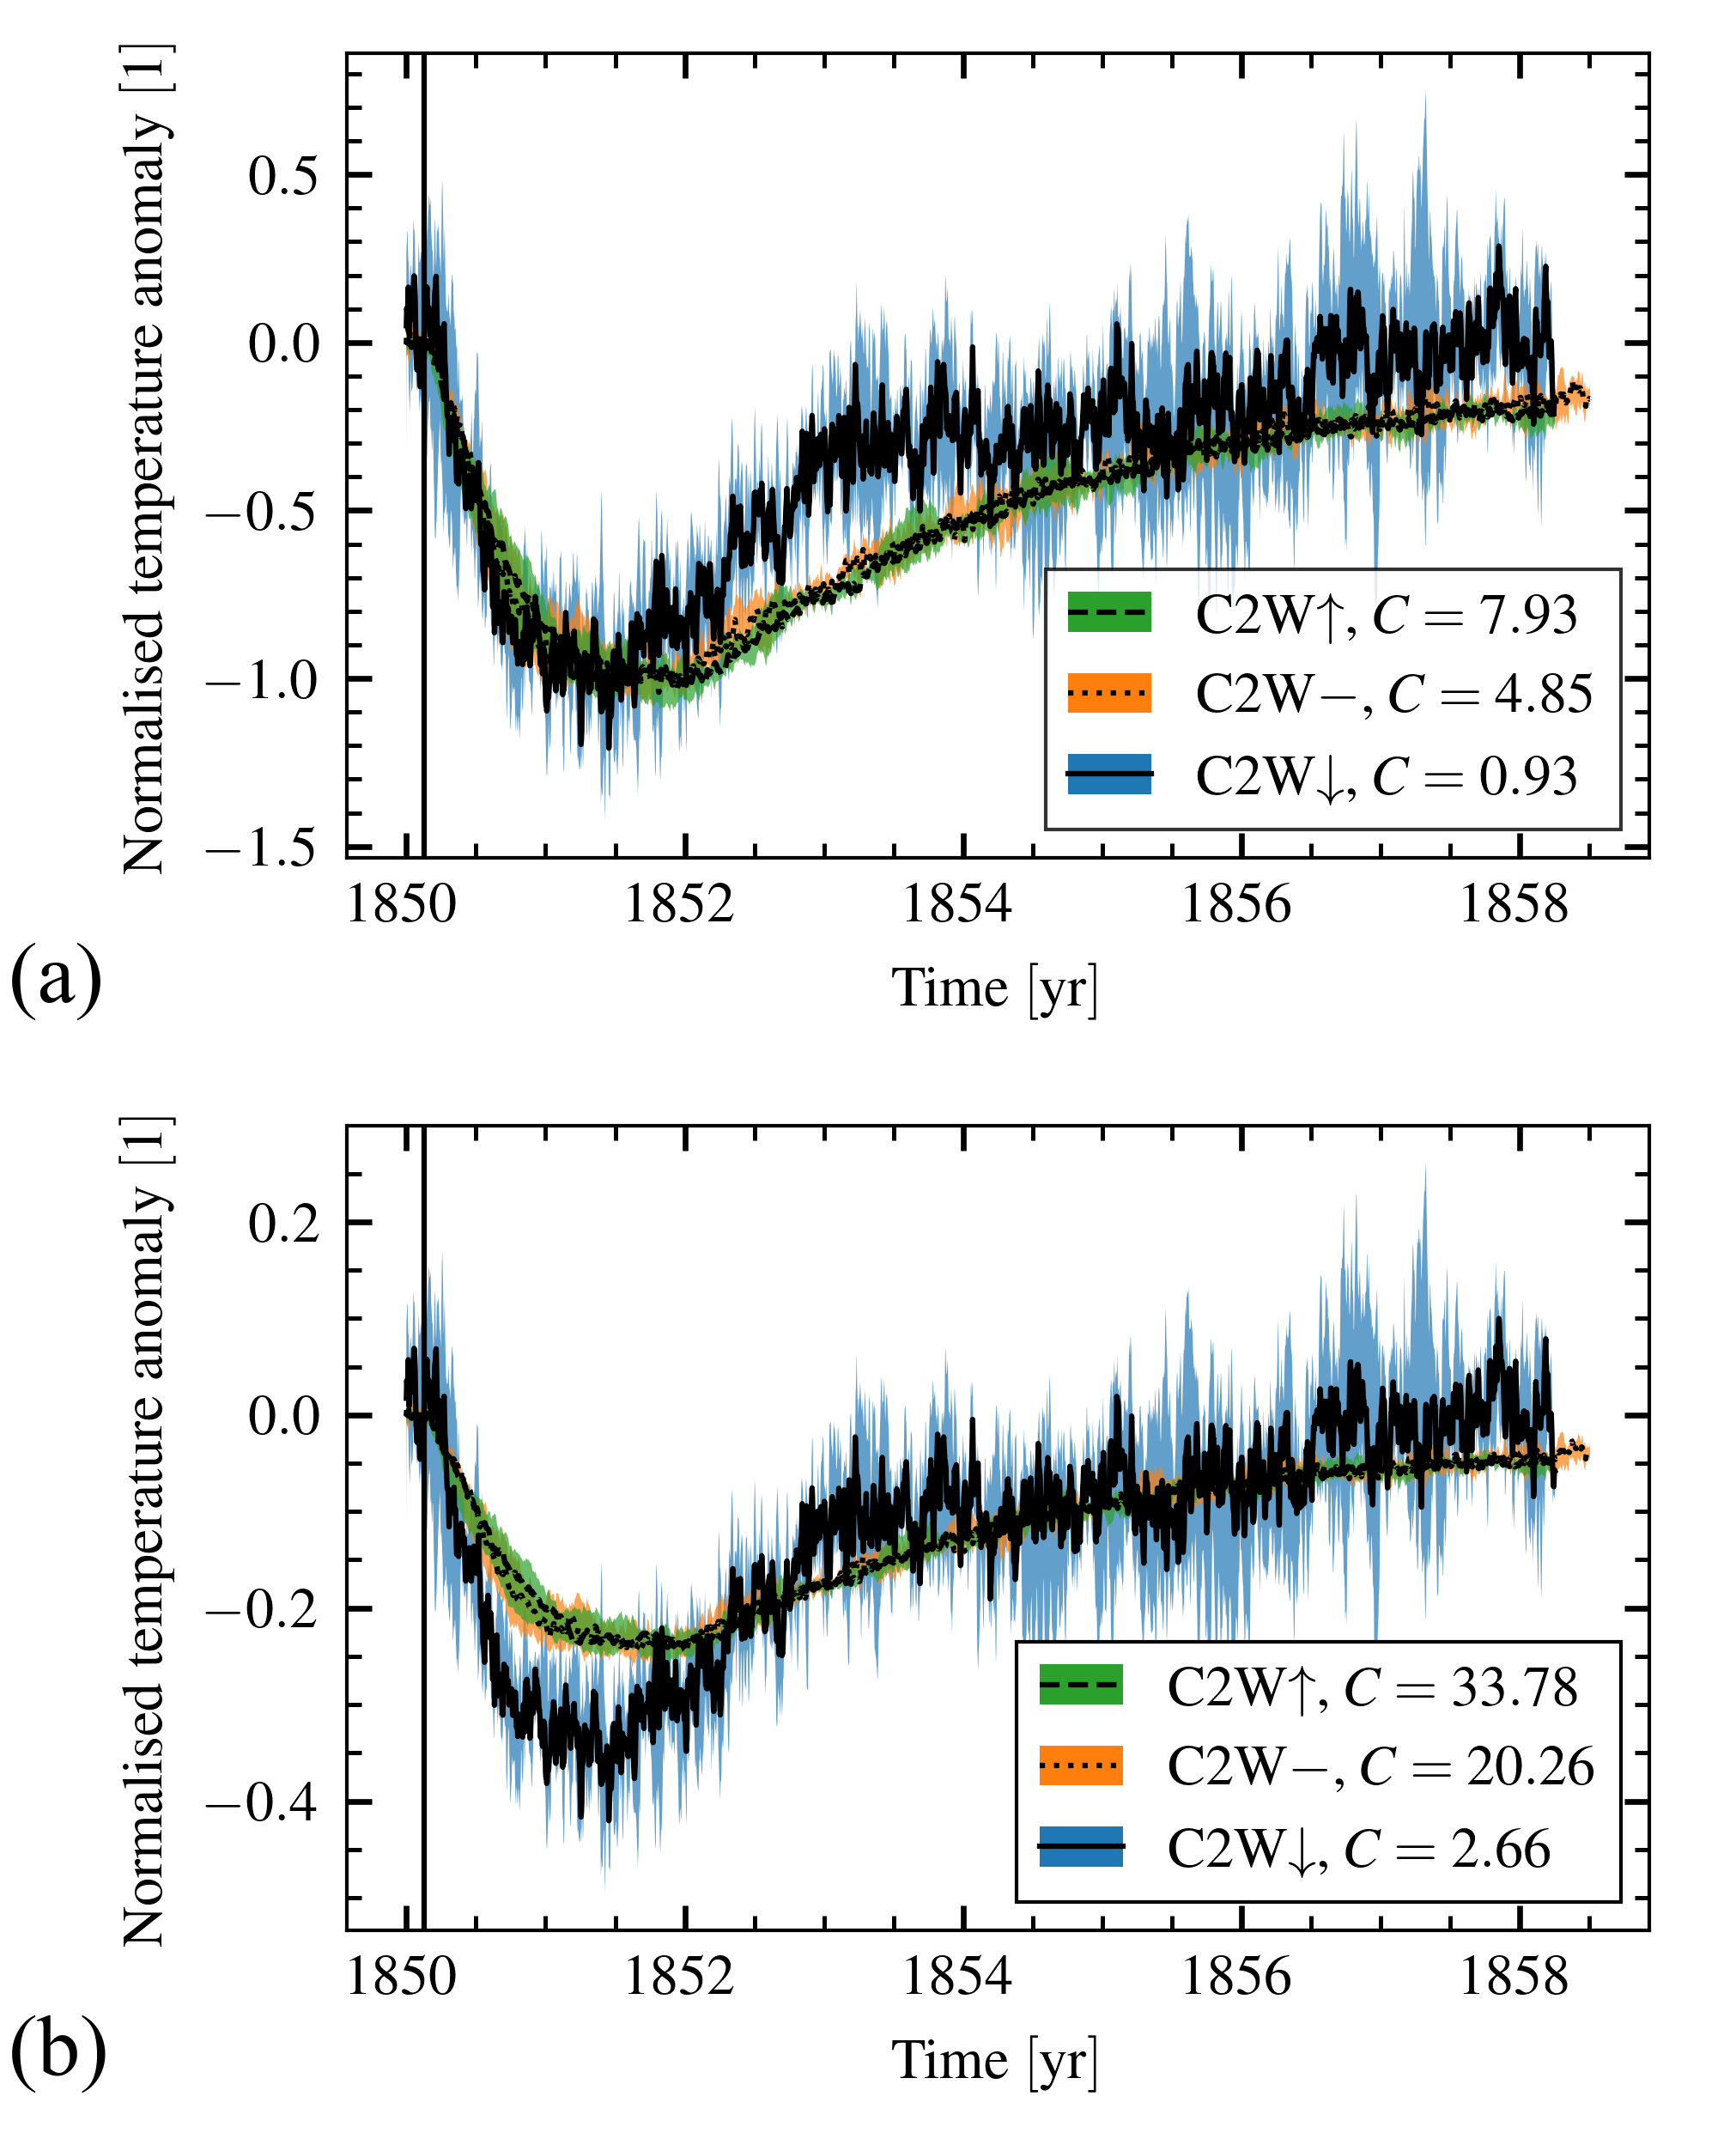
\includegraphics[width=0.95\linewidth]{figures/compare-waveform.png}

  \caption{Temperature response to the three tropical volcanic eruptions cases,
    \gls{c2wm}, \gls{c2wmp} and \gls{c2ws}. The temperature time series have been normalized
    to have (a) peak values at unity and (b) so that they integrate to one, where \(C\) is
    the normalisation constant. Black lines indicate the median across the four member
    ensembles, while shading mark the 5th and 95th percentiles.}\label{fig:compare-waveform}%
\end{figure}

Whether the shape of the temperature time series can be inferred from the shape of
either of the forcing time series (\gls{aod} or \gls{rf}) is a natural question to raise
next. When plotting the \gls{rf} time series, we find that their shapes are consistent
over different eruption strengths (fig.~\ref{fig:arrays_normalised}b), and as such, that
the temperature seem to have a strong dependence on \gls{rf}. The same can largely be
said about the \gls{aod} time series as well, but they do show a slight change in shape
from smaller to larger eruptions (fig.~\ref{fig:arrays_normalised}a). Specifically, the
\gls{aod} time series from the smaller eruptions have a fast rise and a flat peak before
it decays back to its equilibrium state, while from the larger eruptions we find a
slower rise time, but a sharper peak, making the decay to equilibrium happening at a
similar time after the eruption and at a similar rate.
% TODO: Why? Marshall et al. (2019) and references therein may be the best source for a
% suggested explanation.

\begin{figure}
  \centering
  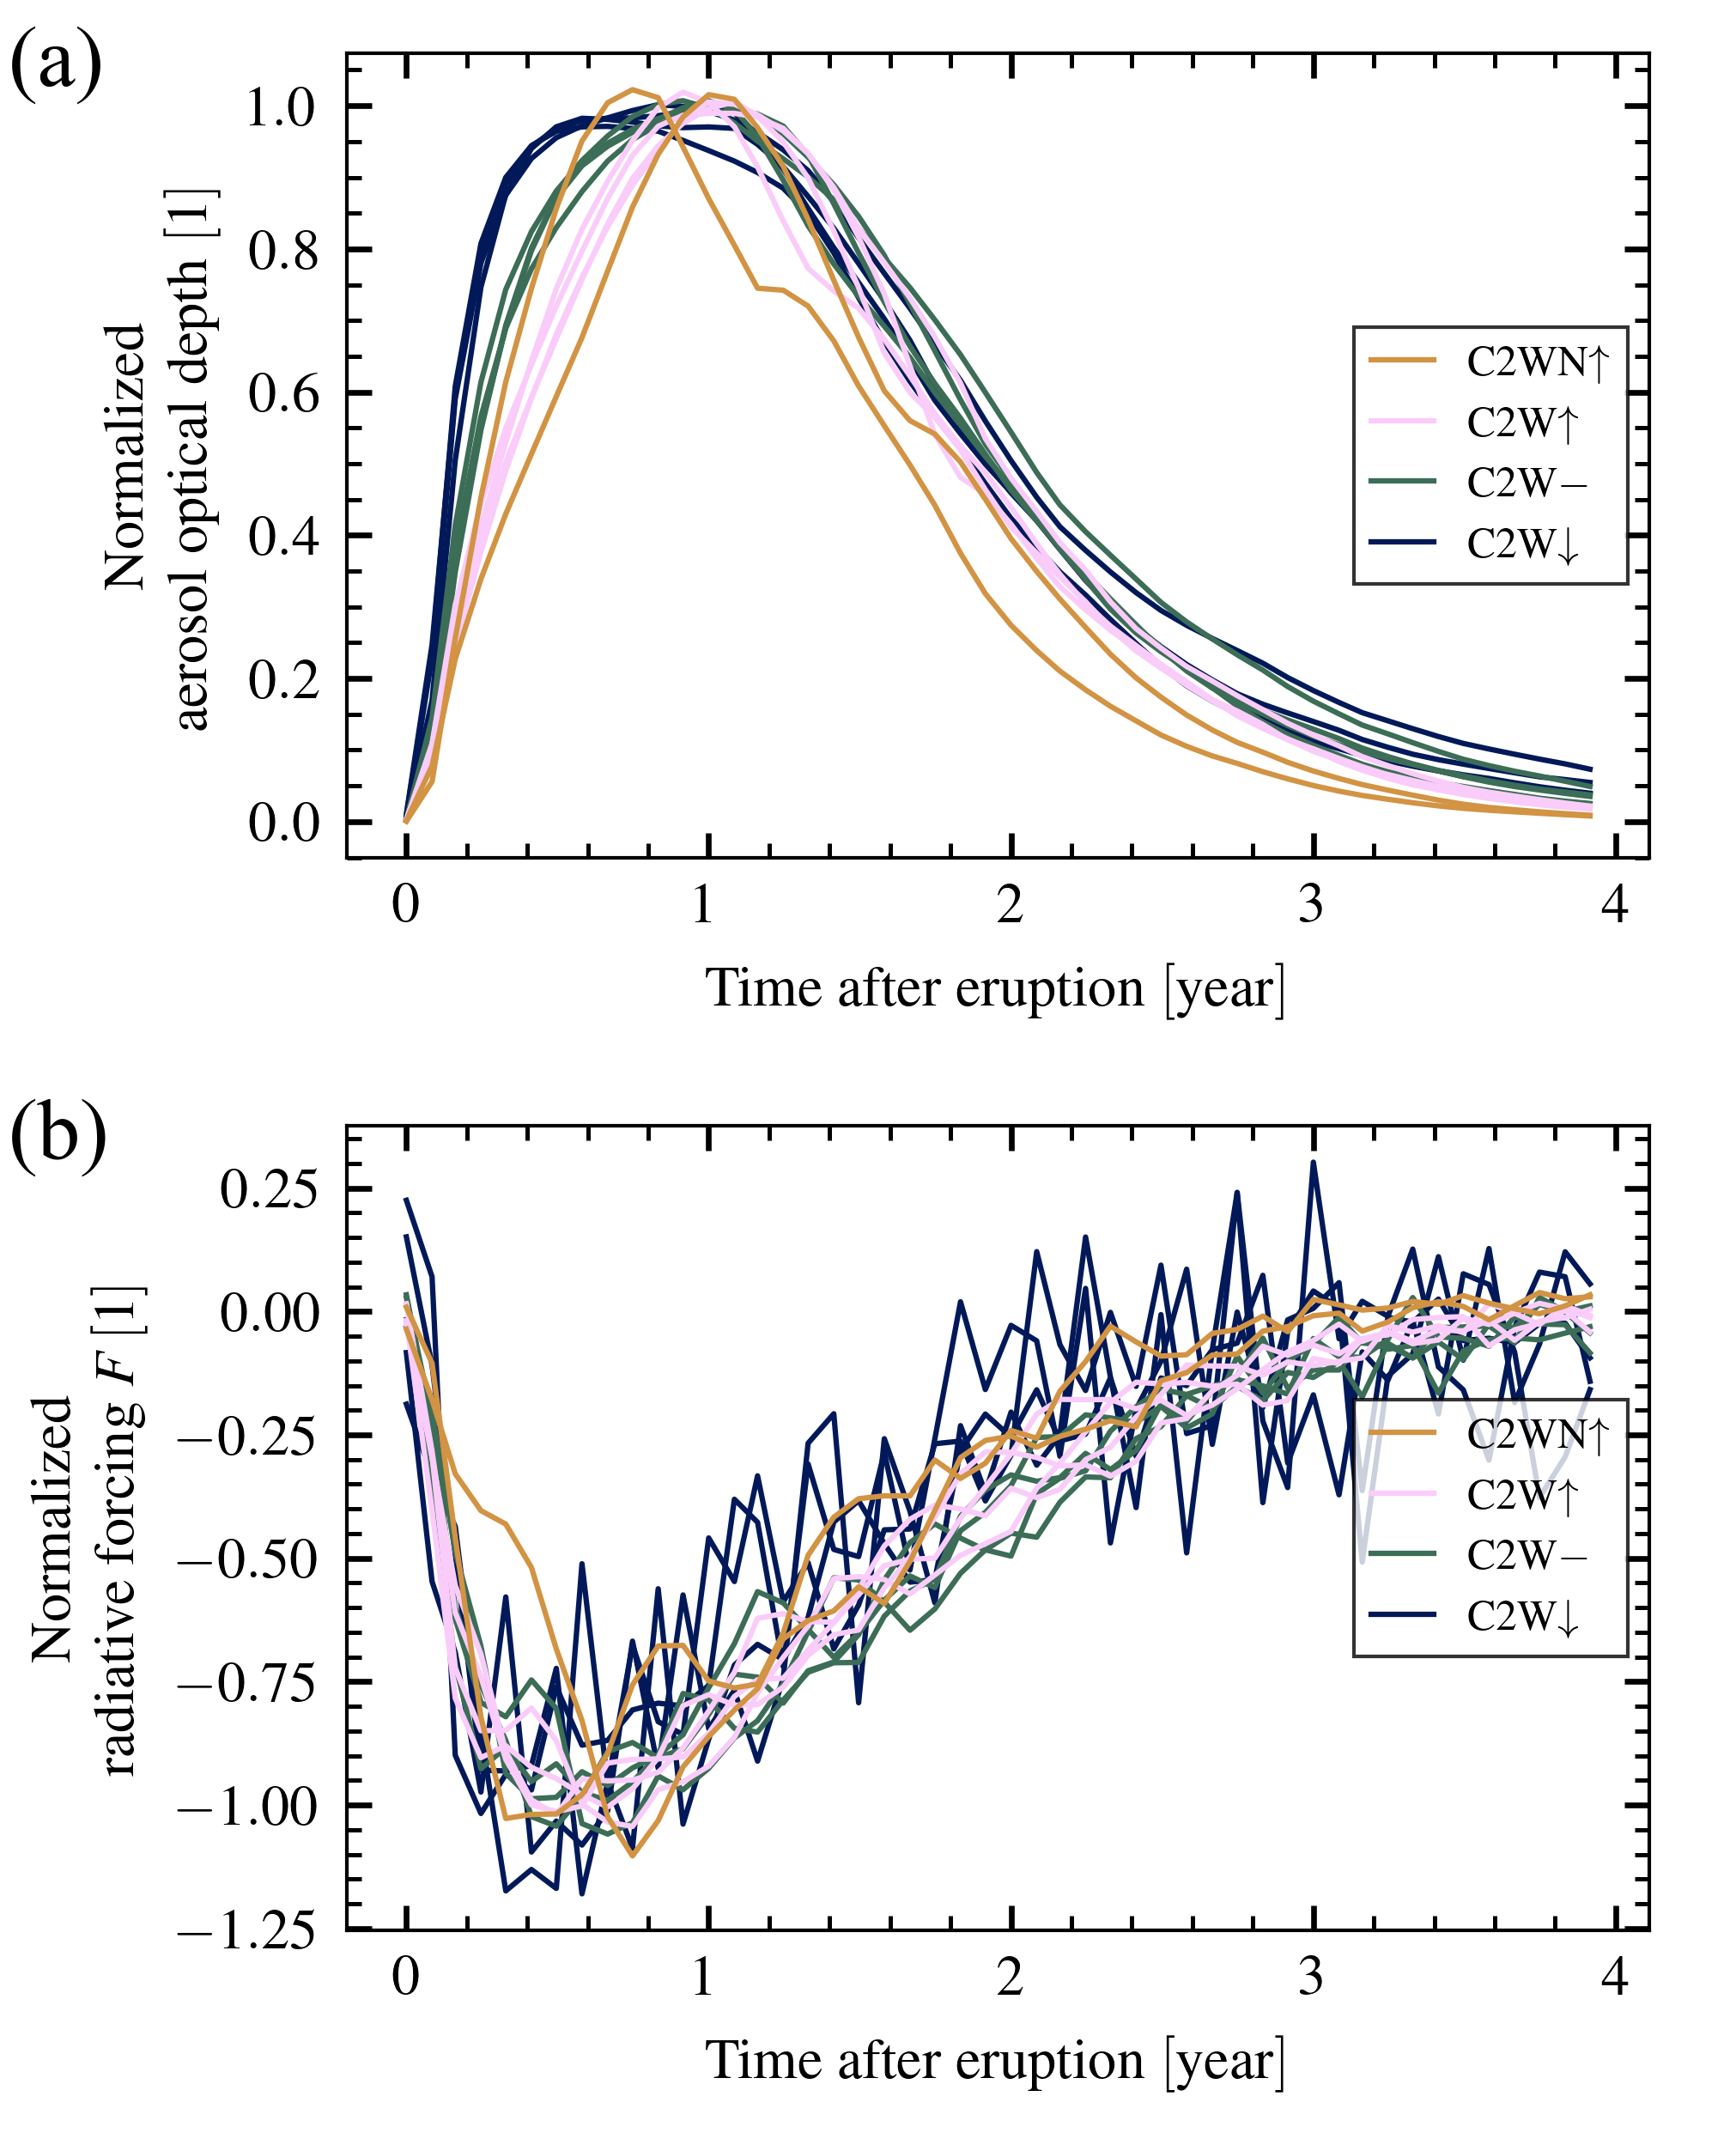
\includegraphics[width=0.95\linewidth]{figures/arrays_combined_normalized.png}

  \caption{The \gls{aod} time series (a) and \gls{rf} time series (b) from the simulations
    summarised in table~\ref{tab:simulation-overview}, scaled to have peak values at unity
  }\label{fig:arrays_normalised}
\end{figure}

\subsection{\gls{rf} dependency on \gls{aod}}

We next focus our attention towards how the \gls{aod} and \gls{rf} time series develop
relative to each other, which are both parameters commonly used for providing insight
about how volcanic eruptions impact climate. A similar comparison was carried out in
\citet[][their Fig.\ 4]{gregory2016} and \citet[][their Fig.\ 1]{marshall2020}, with
\gls{rf} to \gls{aod} plots. Figure~\ref{fig:aod_vs_toa_ses_avg} show annual mean values
from the four simulation cases in table~\ref{tab:simulation-overview}; the small
eruption case (\gls{c2wm}) as blue downward pointing triangles, the intermediate
eruption case (\gls{c2wmp}) as orange thick diamonds, the large tropical eruption case
(\gls{c2ws}) as green upward pointing triangles, the large northern hemisphere eruption
case (\gls{c2wsn}) as brown upward pointing three-branched twigs, and the data from
\citet[][Fig.\ 4, black crosses from HadCM3 sstPiHistVol]{gregory2016} as grey crosses
labelled \glsunset{g16}\gls{g16}. Additionally, the estimated peak values from the Mt.\
Pinatubo and Mt.\ Tambora eruptions are plotted as a purple star and a yellow plus,
while the peak from the \gls{j05} simulation is shown as a pink square. Finally, red
circles represent the peak values obtained from the \gls{c2w} tropical eruption cases.
The gradient lines are the same as shown by \citet{gregory2016}. The full data range is
shown in fig.~\ref{fig:aod_vs_toa_ses_avg}a while fig.~\ref{fig:aod_vs_toa_ses_avg}b
show a narrow range highlighting the \gls{c2wm} case.

The annual mean data from the Pinatubo-like \gls{c2wm} case in
fig.~\ref{fig:aod_vs_toa_ses_avg}b, has \gls{rf} values as a function of \gls{aod} that
follow almost the same constant gradient as the \gls{g16} data. However, in
fig.~\ref{fig:aod_vs_toa_ses_avg}a we find that the stronger eruptions lead to
dissimilar responses in \gls{aod} and \gls{rf}, where the slope of the \gls{c2wmp} case
seem to follow close to a \(-10\) gradient and the \gls{c2ws} case is closer to a \(-5\)
gradient. The peak values (red circles) suggest a non-linear functional shape
dependence, while within each eruption strength the annual mean values fall relatively
close to a straight line.

\begin{figure}
  \centering
  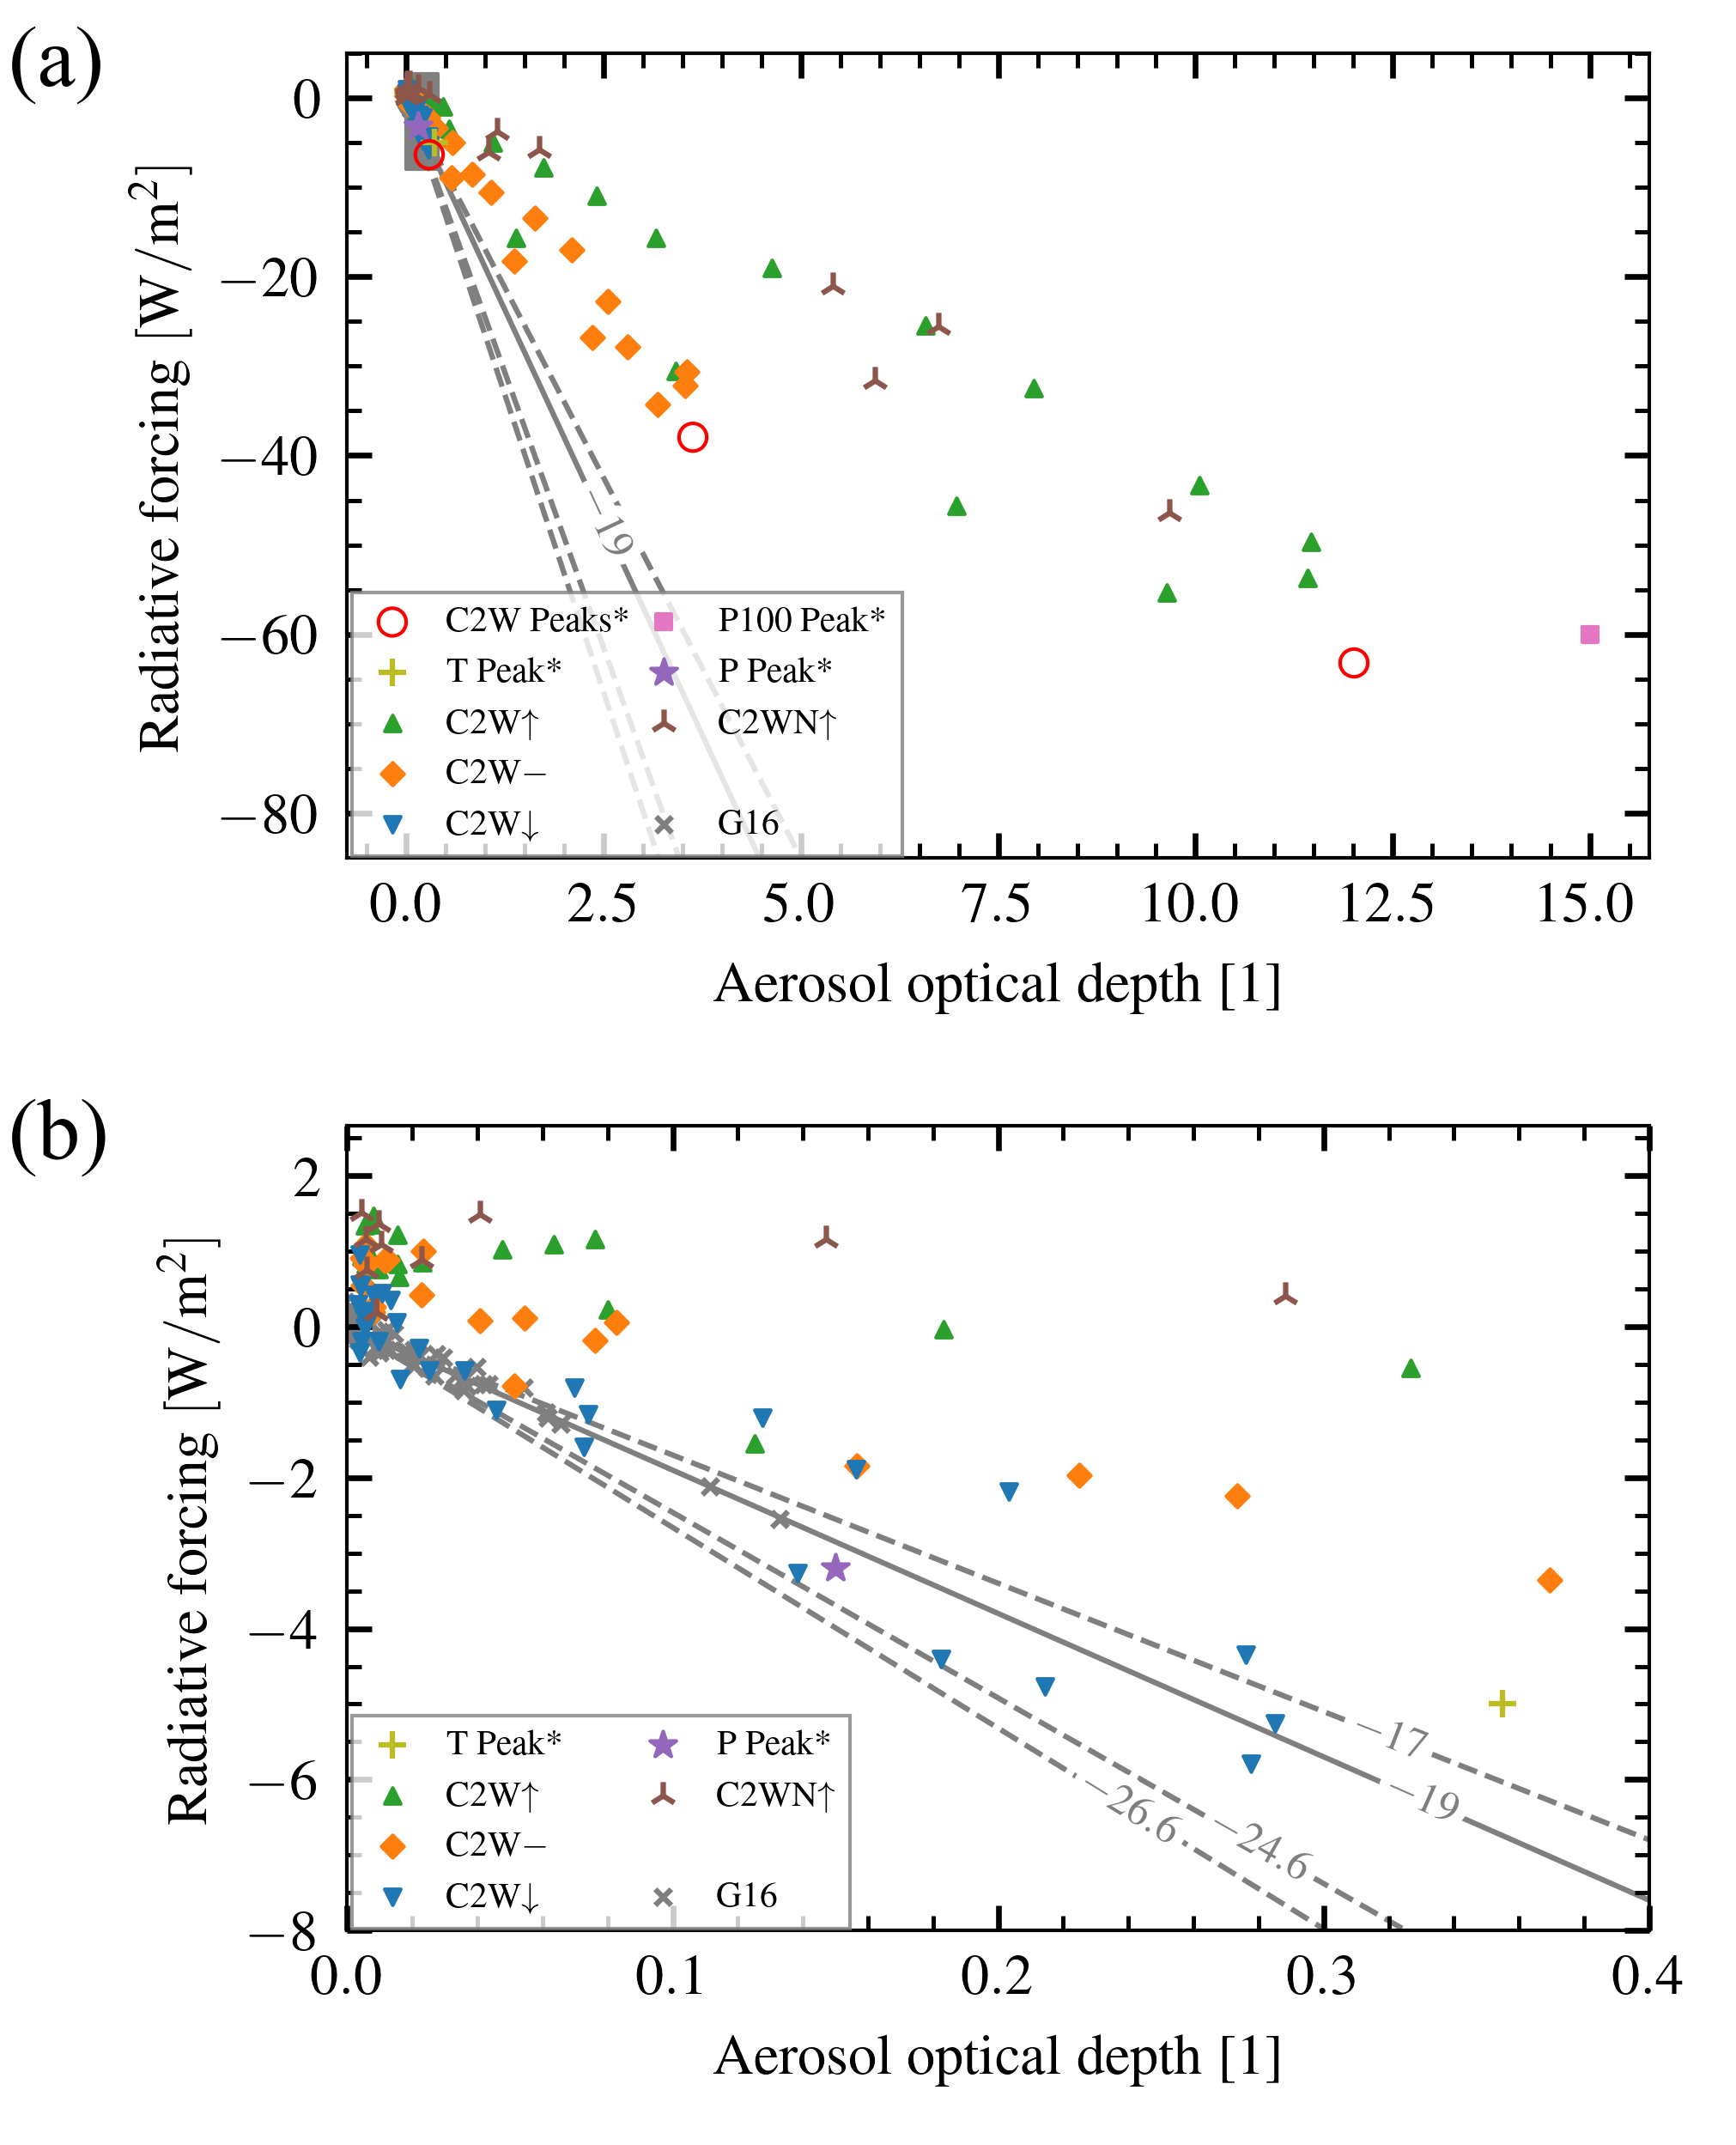
\includegraphics[width=0.95\linewidth]{figures/aod_vs_toa_avg.png}

  \caption{\gls{rf} as a function of \gls{aod}, yearly means. Data from the four
    simulations listed in table~\ref{tab:simulation-overview} (\gls{c2wm}, \gls{c2wmp},
    \gls{c2ws} and \gls{c2wsn}) are shown along with the data from the HadCM3 sstPiHistVol
    simulation by \citet{gregory2016} (grey crosses). Also shown are the estimated peak
    values of the Mt.\ Pinatubo (purple star) and Mt.\ Tambora (yellow plus) eruptions. In
    (a) the simulated super-volcano of \citet{jones2005} (pink square) is shown as well as
    the peak values from the simulations \gls{c2wm}, \gls{c2wmp} and \gls{c2ws} as red
    circles. All peak values (as opposed to annual means) have an asterisk (\(\ast{}\)) in
    their label. The grey gradient lines are the same regression fits as in \citet[][Fig.\
      4]{gregory2016}, where the solid line is the fit to the Gregory et al.\ data (grey
    crosses). (b): Zooming in on the smallest values}\label{fig:aod_vs_toa_ses_avg}%
\end{figure}

To get a feeling for how the responses in \gls{aod} and \gls{rf} develop relative to
each other over time, as briefly mentioned in relation to
fig.~\ref{fig:arrays_normalised}, we plot in fig.~\ref{fig:aod_vs_toa_avg_loop_ratios}
seasonal means of the \gls{rf} to \gls{aod} ratio, where the start of the time series is
taken as that of the eruption day. In fig.~\ref{fig:aod_vs_toa_avg_loop_ratios}a,
straight lines are linear regression fits to the seasonal means across all four
ensembles, summarised in table~\ref{tab:slope-gradients}. Shaded regions are the
standard deviation around the seasonal means. A similar shading is plotted in
fig.~\ref{fig:aod_vs_toa_avg_loop_ratios}b, but where the regression fits have been
omitted to avoid further cluttering the plot. The years where the signal-to-noise ratio
is the lowest are years \(1\) and \(2\), as well as year \(0\) (the noise is mostly due
to the \gls{rf} time series, shown in fig.~\ref{fig:arrays_normalised}b). For this
reason the ratio of \gls{rf} to \gls{aod} is calculated for the second season of the
first year until the end of the third year.

Even though the ratio changes between the eruption magnitudes, we find that the gradient
at which the ratio is changing is similar across large eruption magnitudes, summarised
in table~\ref{tab:slope-gradients}. A slope of approximately \(5.8\) during the first
period is a good fit for both the \gls{c2wmp} case and the \gls{c2ws} case
(table~\ref{tab:slope-gradients}, ``1st period'' and
``fig.~\ref{fig:aod_vs_toa_avg_loop_ratios}a'' columns), and even though the spread in
the \gls{c2wm} case is large in the \(y\)-direction, they tend to follow a similarly
inclined, albeit steeper, slope. Normalizing the time series before computing the ratio,
shown in fig.~\ref{fig:aod_vs_toa_avg_loop_ratios}b, yield a similarly inclined slope
across all forcing magnitude ensembles. In the 2nd period, from the second season of the
second year, the ratios stay close to constant for the reminder of the decaying phase of
the time series. Again this become more clear in the normalized version in
fig.~\ref{fig:aod_vs_toa_avg_loop_ratios}b, where the ratios are similar between the
ensembles.

\begin{table}
  \centering

  \caption{Gradient and standard deviation for the regression lines to the data found in
    fig.~\ref{fig:aod_vs_toa_avg_loop_ratios}. The regression fit in the top row of all
    individual simulations indicate the regression fit to the first period (from year \(0\)
    to year \(1\)), while the bottom is the regression fit to the second period (from year
    \(1\) to year \(3\))}\label{tab:slope-gradients}%
  \begin{tabular}{cccc}
    Figure              & Simulation  & 1st period       & 2nd period       \\
    \multirow{4}{*}{4a} & \gls{c2wsn} & \(1.24\pm1.40\)  & \(-1.32\pm1.01\) \\
                        & \gls{c2ws}  & \(5.26\pm0.49\)  & \(-3.07\pm0.49\) \\
                        & \gls{c2wmp} & \(5.93\pm0.67\)  & \(-2.97\pm0.45\) \\
                        & \gls{c2wm}  & \(11.71\pm2.57\) & \(-1.27\pm1.68\) \\
    \multirow{4}{*}{4b} & \gls{c2wsn} & \(0.22\pm0.25\)  & \(-0.23\pm0.18\) \\
                        & \gls{c2ws}  & \(1.00\pm0.09\)  & \(-0.58\pm0.09\) \\
                        & \gls{c2wmp} & \(0.57\pm0.06\)  & \(-0.29\pm0.04\) \\
                        & \gls{c2wm}  & \(0.52\pm0.12\)  & \(-0.06\pm0.08\) \\
  \end{tabular}
\end{table}

\citet[][their Fig.\ 1c,d]{marshall2020} present results showing a time dependence in
the conversion between \gls{aod} and \gls{rf}, but where \gls{rf} is larger later in the
eruption evolution when compared to \gls{aod} (higher efficiency), not smaller. This is
understood by \citet{marshall2020} to happen since the aerosols are initially spatially
confined to the hemisphere where the eruption was situated, before they during the
second and third years spread globally, leading to a larger global mean albedo per
\gls{aod} and in turn larger \gls{rf} per \gls{aod}. When applying the same analysis as
in fig.~\ref{fig:aod_vs_toa_avg_loop_ratios}a on the \gls{m20} data (used by
\citet{marshall2020}), but only including eruptions between \(-10\) and
\(\SI{10}{\degree\mathrm{N}}\), the ratio increase similarly to the \gls{c2wmp} case
rather than decrease, with slopes of
\(\sim\SI{6.34}{\watt\metre^{-2}\mathrm{AOD}^{-1}}\) and
\(\sim\SI{-0.356}{\watt\metre^{-2}\mathrm{AOD}^{-1}}\) (not shown). The mean ratio for
the tropical \gls{m20} data is similar to the \gls{c2wm} case. From the \gls{m20} data
and the results shown here in fig.~\ref{fig:aod_vs_toa_avg_loop_ratios}, there appear to
be several and competing effects that decide on the values of \gls{aod} and \gls{rf},
but with latitude playing a key role.

The change in ratio, where the smallest ratio is found from the larger eruptions and the
largest ratio is from the smaller eruptions, is consistent with the change in peak
values seen in fig.~\ref{fig:aod_vs_toa_ses_avg}a, where the red circles indicate that
the peak values are saturating in \gls{rf}. The \gls{rf} peak magnitudes increases more
slowly than the \gls{aod} peak magnitudes, which increases close to linearly with
injected \ce{SO2} (see also fig.~\ref{fig:parameter_scan}a). This may be the result of
larger aerosols having time to develop as the amount of injected \ce{SO2} increases
\citep{niemeier2015,marshall2019}. This in turn make the forcing from smaller eruptions
more efficient than from large eruptions since larger aerosols scatter radiation less
efficiently, causing a smaller \gls{rf} to \gls{aod} ratio.

\begin{figure}
  \centering
  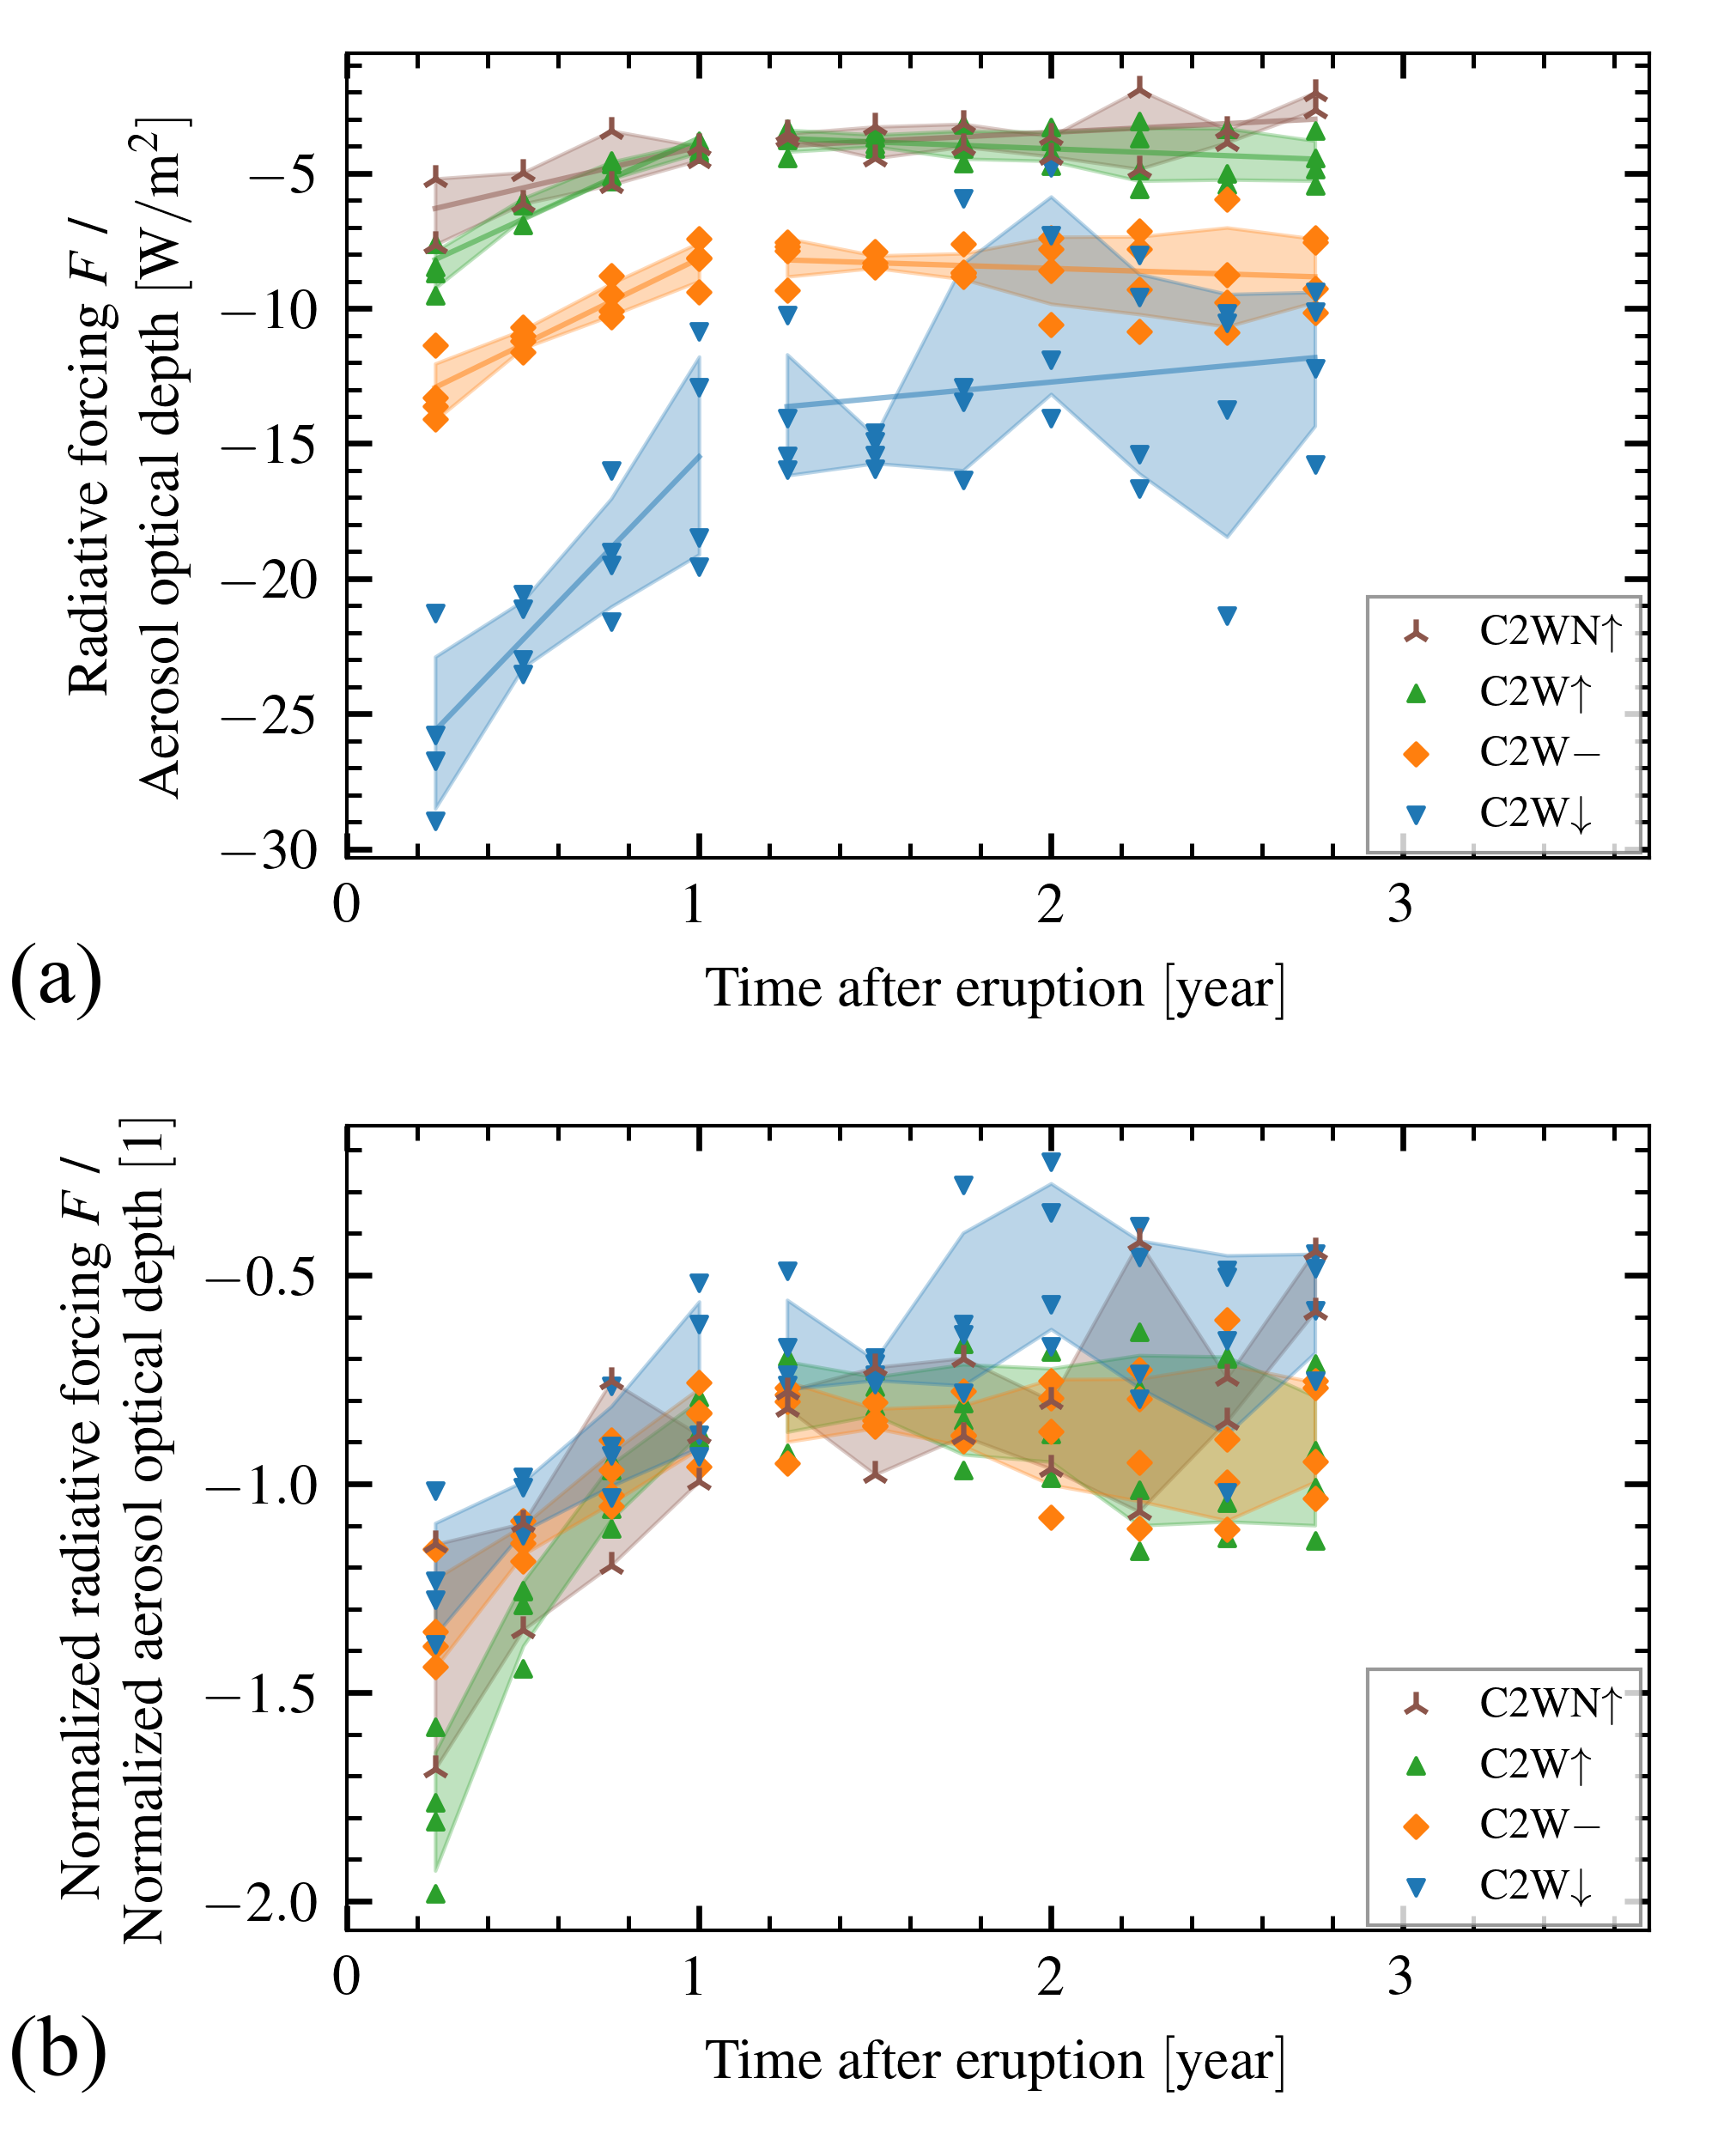
\includegraphics[width=0.95\linewidth]{figures/aod_vs_toa_loop.png}

  \caption{(a): Ratio of \gls{rf} to \gls{aod}, with time-after-eruption on the horizontal
    axis. Slopes are linear regression fits and are described in
    table~\ref{tab:slope-gradients}, while shaded regions are the standard deviation across
    the ensembles for each season. (b): Same as in (a), but where the underlying \gls{aod}
    and \gls{rf} time series have been scaled to have peak values at
    unity}\label{fig:aod_vs_toa_avg_loop_ratios}%
\end{figure}

\subsection{Parameter scan}

In fig.~\ref{fig:parameter_scan} we compare all relevant parameters to each other. The
initial input parameter to the \gls{cesm2} is injected \ce{SO2}. Compared to \gls{aod}
peak values we get an almost linear relationship against \iso{} for our tropical cases
(\gls{c2w}), shown in fig.~\ref{fig:parameter_scan}a. The latitude also play a role for
how large the \gls{aod} perturbation becomes, as we can see from the \gls{c2wsn} data
point. A weak dependence on eruption latitude is also reported in \citet{marshall2019},
where they find \(\SI{72}{\percent}\) of the \gls{aod} variance can be explained by
\iso{}, while latitude contributes to only \(\SI{16}{\percent}\) of the variance. Peak
values from their data (82 simulations) is plotted as green thin diamonds and show a
similar pattern, where \gls{aod} depends close to linearly on \iso{}, but where latitude
give a spread in \gls{aod}. Peak values from Mt.\ Pinatubo (P) and Mt.\ Tambora (T) are
show for reference, along with peak values from \gls{j05} and \gls{t10}.

With the almost linear relation between \iso{} and \gls{aod} for the \gls{c2w} data, we
should expect to see a similar plot for \iso{} versus \gls{rf} as for \gls{aod} versus
\gls{rf}. \iso[I] versus \gls{rf} is shown in fig.~\ref{fig:parameter_scan}b, but where
the absolute value of the \gls{rf} is potted along the \(y\)-axis. Just as in
fig.~\ref{fig:aod_vs_toa_ses_avg}a we find the \gls{c2w} data points to be heavily
damped in \gls{rf} as \iso{} increases. The same effect can be seen in the data from
\gls{ob16} (red downward triangles), which follow much the same path as our tropical
cases. A description of how the \gls{ob16} data was analysed can be found in the
appendix. The simulations used by \citet{ottobliesner2016} was using the \gls{cesm1}
with a low-top atmosphere (\gls{cam5}), thus we find that despite the difference in
model complexity, similar \glspl{rf} are obtained by \citet{ottobliesner2016} as what we
find.

\begin{figure*}
  \centering
  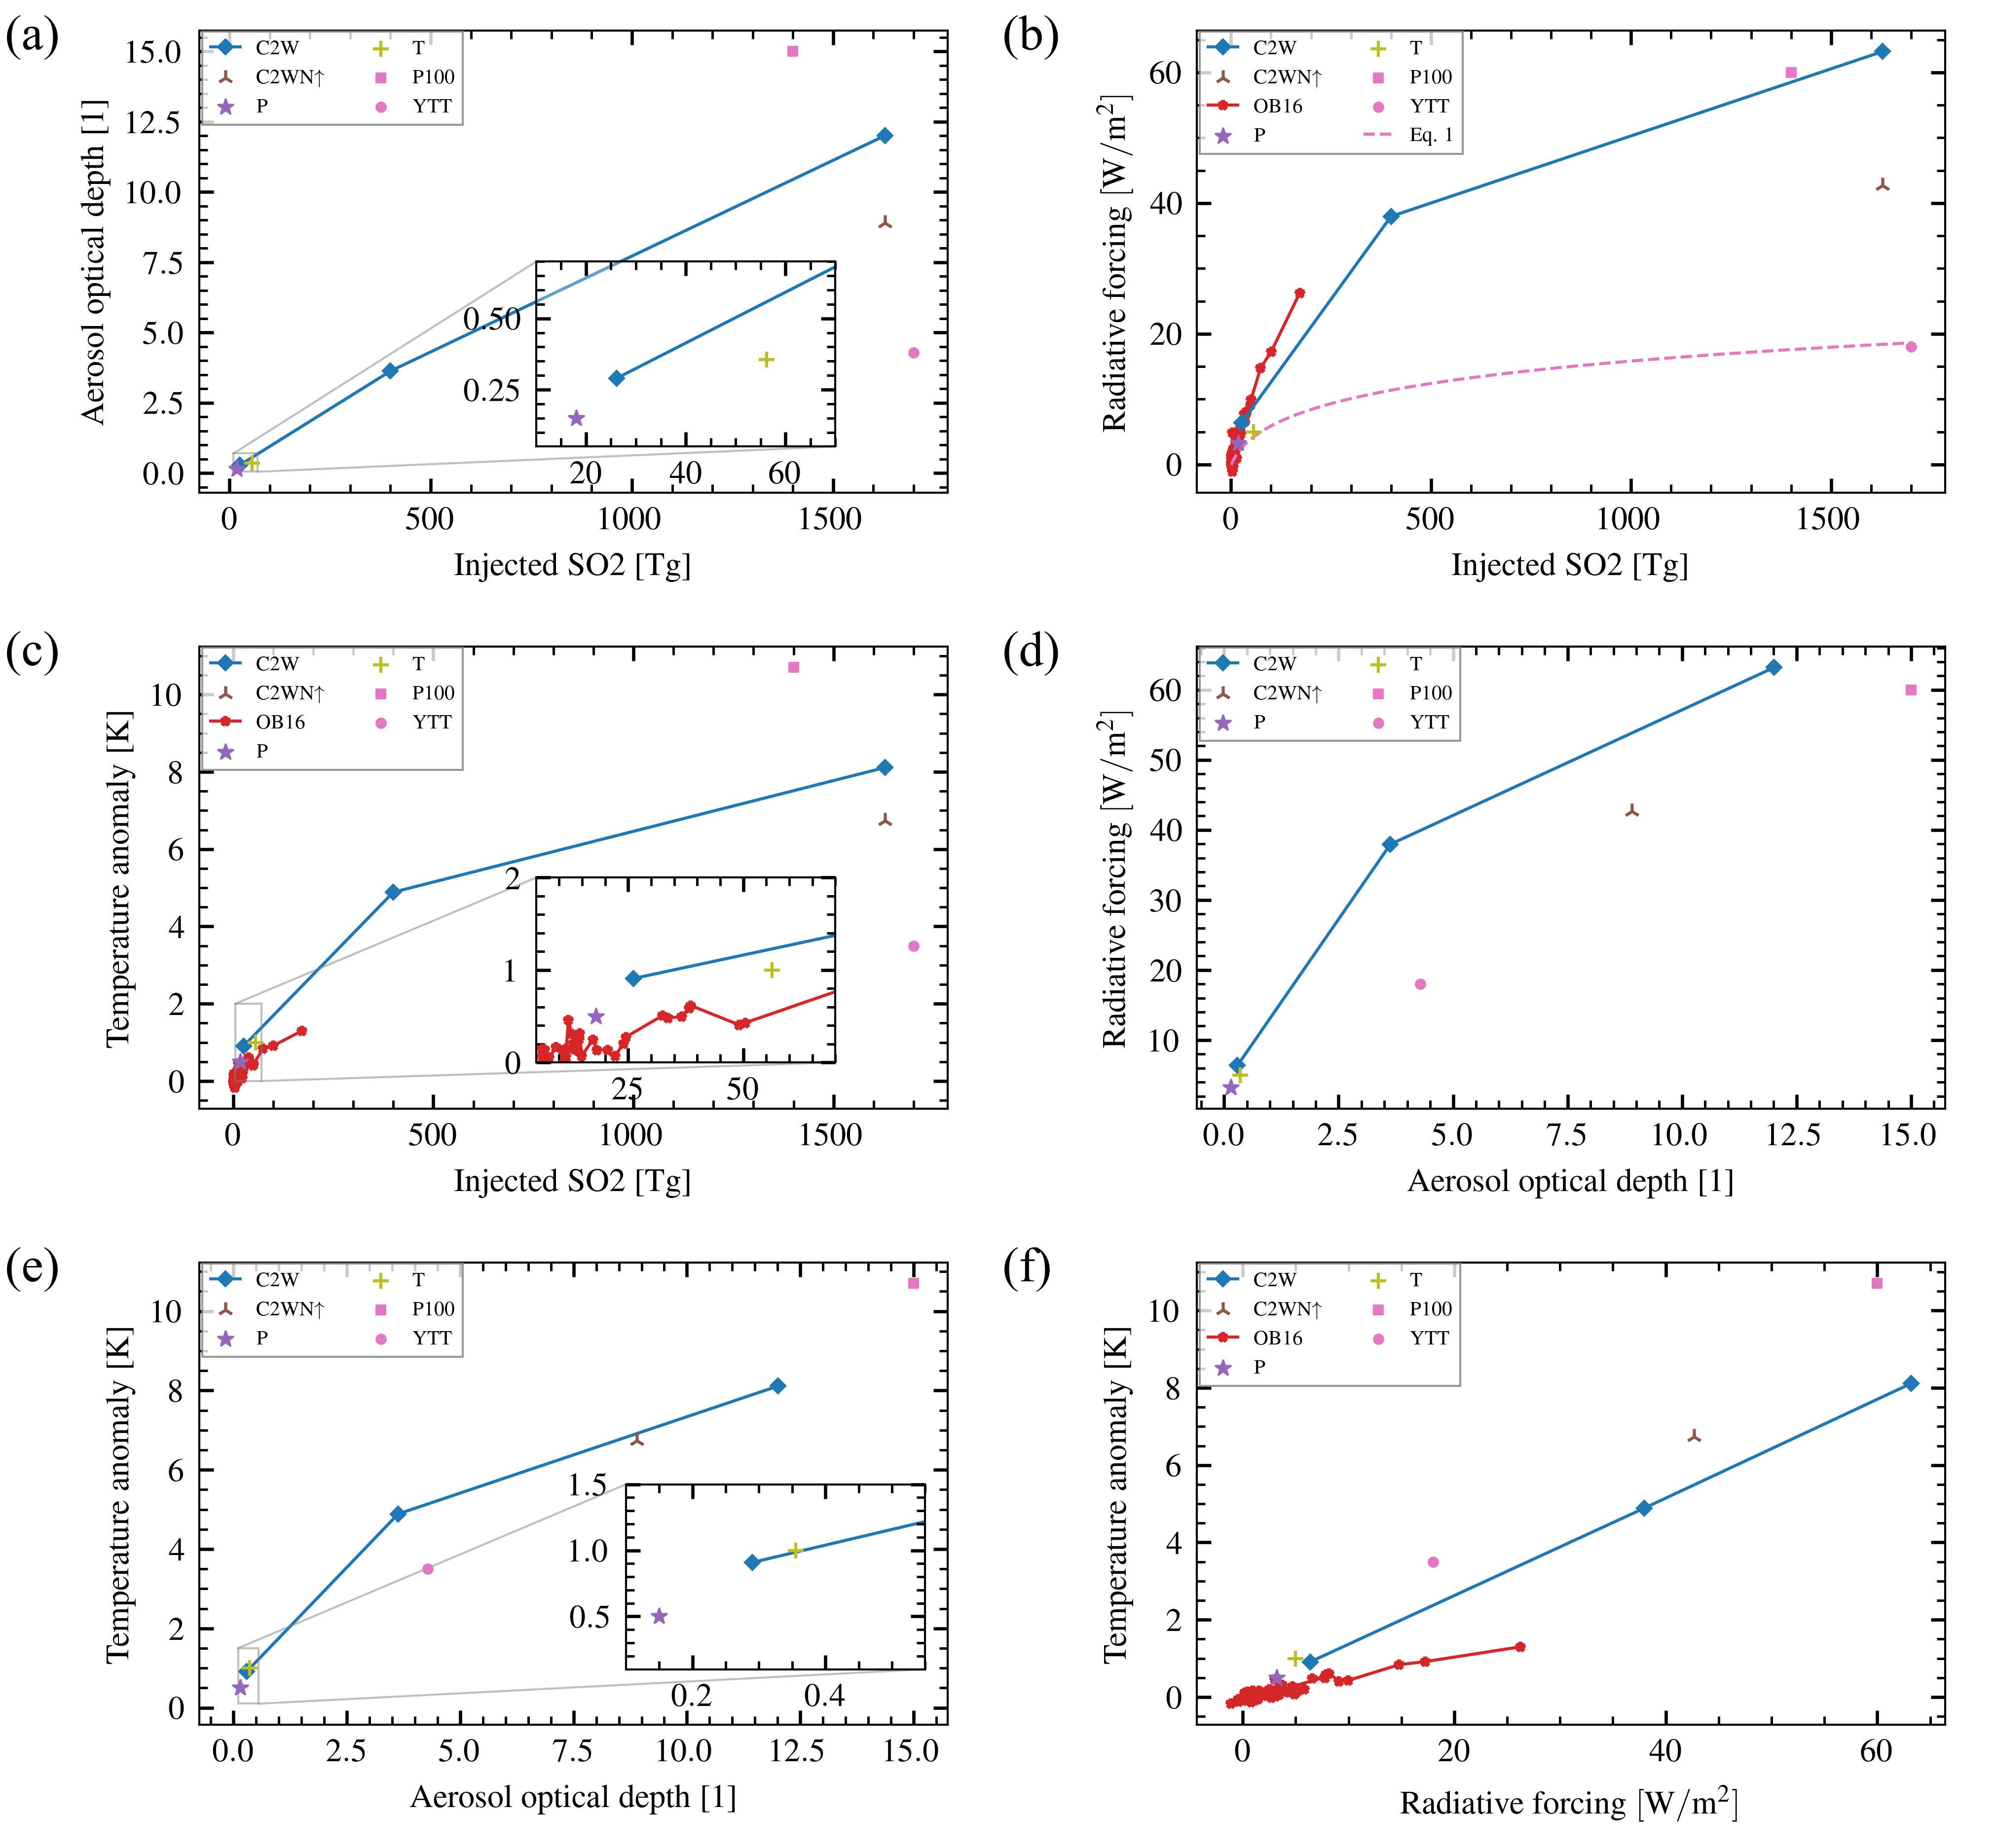
\includegraphics[width=0.95\linewidth]{figures/parameter_scan.png}

  \caption{(a) \gls{aod} (b) \gls{rf} and (c) temperature as a function of \iso{}\@. (d)
    \gls{rf} and (e) temperature as a function of \gls{aod}. (f) Temperature as a function
    of \gls{rf}. Tropical cases (\gls{c2wm}, \gls{c2wmp}, \gls{c2ws}) are shown as blue
    diamonds labelled \gls{c2w}, the \gls{c2wsn} case is the brown three-branched twig,
    \gls{ob16} are data from \citet{ottobliesner2016} marked with red downward triangles,
    while green thin diamonds labelled \gls{m20} show the \citet{marshall2020dataset} data.
    The purple star and yellow plus are Mt.\ Pinatubo and Mt.\ Tambora estimates based on
    observations, the pink square labelled \gls{j05} is the one-hundred times Mt.\ Pinatubo
    super-volcano from \citet{jones2005} and the pink disk labelled \gls{t10} is the
    \gls{ytt} super-volcano from \citet{timmreck2010}. The pink dashed line labelled N15 is
    from \citet{niemeier2015} and show the functional given in
    eq.~\ref{eq:niemeier_exponential}}\label{fig:parameter_scan}%
\end{figure*}

% INFO: the conversion between S and SO2 is confirmed by Niemeier and Timmreck (2015)'s
% reference to the Bekki et al. (1996) paper. Bekki uses 6000 Mt SO2, Niemeier uses 3000
% Tg(S).
\citet{niemeier2015} did simulations of continually emitting injections of sulphur, up
to \(\SI{200}{\tera\gram(\ce{SO2})\mathrm{yr}^{-1}}\), in the middle atmosphere version
of the ECHAM5 \citep{giorgetta2006} climate model and with aerosol microphysics from HAM
\citep{stier2005}. They found that the impact of increasing the injection rate lead to
an \gls{rf} as a function of injection rate \(x\) that had an exponential decay
converging to \(\SI{-65}{\watt\meter^{-2}}\),
\begin{equation}
  \Delta
  R_{\mathrm{TOA}} =
  -\SI{65}{\watt\metre^{-2}}
  \mathrm{e}^{-{\left(\frac{\SI{2246}{\tera\gram(S)yr^{-1}}}{x}\right)}^{0.23}}.
  \label{eq:niemeier_exponential}
\end{equation}
This is shown in fig.~\ref{fig:parameter_scan}b as the stippled pink line to have a much
slower rise than the data from both our simulations and the simulations by
\citet{ottobliesner2016}. However, \citet{timmreck2010} did simulations in the MPI-ESM
that was forced with \gls{aod} obtained from the HAM aerosol model, of a
\(\SI{850}{\tera\gram(\ce{S})}\) eruption representing the \gls{ytt} eruption. That is,
the same aerosol microphysical model was used in \citet{timmreck2010} and
\citet{niemeier2015}, as well as very similar \glspl{esm}; the MIP-ESM is the ancestor
of ECHAM6 which was the next version update from ECHAM5 \citep{kuma2023}. From the
initial input of \(\SI{850}{\tera\gram(\ce{S})}\) (equivalent to
\(\SI{1700}{\tera\gram(\ce{SO2})}\)), via an \gls{aod} estimate, they got a peak
\gls{rf} of \(\SI{-18}{\watt\metre^{-2}}\) (pink filled circle in
fig.~\ref{fig:parameter_scan} labelled \gls{t10}). This is in good agreement with the functional given in
eq.~\ref{eq:niemeier_exponential}. Interestingly, we also find that the peak values from
the \gls{m20} data are nicely bounded by the \gls{cesm} data (\gls{c2w} and \gls{ob16})
from above and eq.~\ref{eq:niemeier_exponential} from below. The eruptions close to
equator give the data points close to the upper bound while the eruptions at higher
latitudes give weaker \gls{rf} peak values down to the lower bound.

Figure~\ref{fig:parameter_scan}c show \iso{} versus temperature response. Just as in
fig.~\ref{fig:parameter_scan}b, the data from the \gls{c2w} cases bend off, making the
temperature response weaker with higher values of \iso{}. We find here that the
\gls{ob16} data follow a different path than the \gls{c2w} data, with temperature
fluctuations being less extreme as \iso{} increases. \gls{t10} also find a much weaker
temperature response than our results suggest, with a maximum temperature perturbation
of only \(\SI{-3.5}{\kelvin}\) for their \(\SI{1700}{\tera\gram(\ce{SO2})}\) eruption,
while the opposite is the case for the \gls{j05} simulation which resulted in a maximum
temperature perturbation of \(\SI{-10.7}{\kelvin}\), much greater than what we obtain in
our \gls{c2w} simulations.

In fig.~\ref{fig:parameter_scan}d we again look at \gls{rf} as a function of \gls{aod},
but this time focus on the peak values rather than the annual and seasonal means. As
previously discussed, the \gls{rf} to \gls{aod} ratio is much weaker than what previous
studies have found, and the \gls{c2w} cases give peak values that do not follow a
straight line. Comparison with the results from other studies \citep{jones2005,
  marshall2020, timmreck2010} suggests that there might be large dependencies on the model
that was used as well as on the input parameters of the model, for example related to
latitude. These contributions add on top of noise, which for the relatively small
ensemble size of four used here may play a role.

Figure~\ref{fig:parameter_scan}e should in the case of the \gls{c2w} data be akin in
shape to the paths found in fig.~\ref{fig:parameter_scan}c due to the close to linear
relationship found between \iso{} and \gls{aod} in fig.~\ref{fig:parameter_scan}a. The
relationship between \gls{aod} and temperature do tend to follow a similar functional
shape, but more data would be needed to draw strong conclusions from this. The
similarities between the \gls{m20} data in figs.~\ref{fig:parameter_scan}c and
\ref{fig:parameter_scan}e are apparent, but it is worth noting that these were run with
prescribed sea surface temperatures, preventing the surface temperature from being fully
perturbed.

In fig.~\ref{fig:parameter_scan}f we compare the \gls{rf} and temperature responses.
Both the \gls{c2w} data and the \gls{ob16} data show a close to linear relationship
between temperature and \gls{rf}, but where the \gls{c2w} data has a steeper gradient
and as such seem to lead to stronger temperature perturbations compared to \gls{ob16}.
However, the overlap in data is not big, and the \gls{c2w} data are too sparse to make
strong conclusions, in addition to the difference in model complexity. It is also
important to note that the temperature values used in the \gls{ob16} data points are the
exact temperature at day 400 (ca.\ 13 months) after the eruption according to the \iso{}
time series. Thus, missing the peak temperature means the estimates will be biased
towards lower temperatures, while other eruptions occurring close in time will
contribute a bias to higher temperatures. This, in combination with strong noise make
the \gls{ob16} data less reliable.

\section{Discussion}\label{sec:discussion}

% NOTE: Suggested layout for the
% Discussion:
% - Explain the results and emphasize significant findings clearly
% - Discuss the impact and importance of results compared with recent relevant research
% Conclusion
% - The justification for these objectives: Why is the work important?
% - Summarize the key points made in the other sections
% - Conclude overall discussion of article
% - Link this section to the introduction

\subsection{Linearity between \gls{aod} and \gls{rf}}

Figures~\ref{fig:aod_vs_toa_ses_avg},~\ref{fig:aod_vs_toa_avg_loop_ratios} and
\ref{fig:parameter_scan}d all indicate that as the \gls{aod} increases past \(\sim
1.0\), the scaling of \(\sim \SI{-20}{\watt\metre^{-2}\mathrm{AOD}^{-1}}\) no longer map
to corresponding values of \gls{rf}. Looking at the intermediate volcanic eruption with
\(\SI{400}{\tera\gram(\ce{SO2})}\) (\gls{c2wmp}) there seem to be a mostly linear
relationship between the \gls{aod} and \gls{rf} values, with a slope of approximately
\(\SI{-10}{\watt\metre^{-2}\mathrm{AOD}^{-1}}\). As for the largest eruption, scaling
\gls{aod} by \(\sim \SI{-5}{\watt\metre^{-2}\mathrm{AOD}^{-1}}\) yields reasonable
\gls{rf} values. From fig.~\ref{fig:parameter_scan}a we have an almost linear relation
between \iso{} and \gls{aod}. Previous results indicate that larger eruptions where more
\ce{SO2} is injected creates larger aerosols which are less effective at scattering
radiation, making the cooling less efficient
\citep{english2013,timmreck2010,timmreck2018}, an effect seen to influence the \gls{rf}
and not \gls{aod}.

\citet{timmreck2010} also remark that for very large eruptions, they look at Mt.\
Pinatubo and \gls{ytt}, \ce{OH} radicals are not abundant enough which limit the
\ce{SO2} oxidation. The peak in \gls{aod} levels for the \gls{ytt} simulation appear six
months after the peak of Mt.\ Pinatubo in \citet{timmreck2010}, and at a much smaller
value when compared to a \(100\times\) scaling, see their Fig.\ 1c, similar to what was
found here and shown in fig.~\ref{fig:arrays_normalised}a where \gls{aod} peaks earlier
for smaller eruptions. \citet{timmreck2010} obtain a peak \gls{rf} anomaly of
\(\SI{-18}{\watt\metre^{-2}}\) (\(7\)-\(8\) months after) compared to \citet{jones2005}
of \(\SI{-60}{\watt\metre^{-2}}\) (one year after). \gls{rf} peak occurring before the
\gls{aod} peak is again the same as what has been found here for \gls{cesm2},
approximately \(6\)--\(8\) months after the eruption (see
fig.~\ref{fig:arrays_normalised}). The magnitude of the \gls{rf} peak is much smaller in
\citet{timmreck2010} than what we find, but does correspond well with both the
functional fit obtained by \citet{niemeier2015} and the lower bounds from eruption
simulations done by \citet{marshall2020}. As such, it is clear that the \gls{aod} time
series are dependant on the magnitude of \iso{} to the extent of the timing of the peak,
while the \gls{rf} time series are similar in shape but with smaller relative magnitudes
as the \iso{} increases.

While the \gls{j05} data is comparable to the \gls{c2ws} simulation case in both
\gls{aod} and \gls{rf}, the temperature response reported by \citet{jones2005} is much
stronger than what our strongest eruption produce. Since \citet{jones2005} used the
\gls{aod} forcing from Mt.\ Pinatubo multiplied by one hundred, the shape of the time
series is notably different to what a super-eruption would create. This might be enough
to cause a much stronger temperature perturbation. We also note that
\citet{timmreck2010} used a more realistic \gls{aod} forcing and obtained cooling that
was much smaller than \citet{jones2005}.

The biggest spread is found when converting from \iso{} to any of the three output
parameters when comparing across models. Conversion from \iso{} to \gls{aod} is
consistent within similar models, even when comparing simulations of volcanic eruptions
\citep{timmreck2010} and continuous injection of \ce{SO2} \citep{niemeier2015}, but has
a wide spread at large values of \iso{} across models
(figs.~\ref{fig:parameter_scan}a,b,c). Compared to \gls{aod} as a function of \iso{},
both \gls{rf} (fig.~\ref{fig:parameter_scan}d) and temperature
(fig.~\ref{fig:parameter_scan}e) as a function of \gls{aod} result in a small spread in
the data across models, and necessarily the spread will also be small for temperature as
a function of \gls{rf} (fig.~\ref{fig:parameter_scan}f). A roughly linear relationship
between \gls{aod} and \gls{rf} have been assumed is several previous studies, but (1)
for smaller values of \gls{aod} and \gls{rf}, and (2) where the estimated slope is
significantly steeper; around \(\SI{-20}{\watt\metre^{-2}\mathrm{AOD}^{-1}}\) at
\(\mathrm{AOD}<1\) rather than \(\sim\SI{-5}{\watt\metre^{-2}\mathrm{AOD}^{-1}}\) found
here at \(\mathrm{AOD}\gg1\). We therefore expect a linear relationship to be a precise
estimate of the \gls{rf} dependence on \gls{aod} for eruptions of the same magnitude or
less than Mt.\ Pinatubo. For larger eruptions, lack of \ce{OH} and aerosol growth
affecting both reflectance and their gravitational pull, significantly influence both
the \gls{aod} and \gls{rf} evolution.

From the \gls{c2w} cases in particular, there appear to be a time-after-eruption
dependency on the \gls{rf} to \gls{aod} ratio. \citet{marshall2020} discuss the same
feature, but find when looking at \gls{aod} and \gls{rf} that the efficiency increases
from year 1 to year 2, while here efficiency decreases with time, as shown in
fig.~\ref{fig:aod_vs_toa_avg_loop_ratios}. \citet{marshall2020} explain that this is due
to the time it takes for the aerosols to spread which affects the global albedo and in
turn the \gls{rf}, with the \gls{aod} being less affected by the aerosols spreading.
However, when looking only at the tropical eruptions in \gls{m20} (between \(-10\) and
\(\SI{10}{\degree\mathrm{N}}\)), the \gls{rf} to \gls{aod} ratio become
indistinguishable to what found here from the \gls{c2wmp} simulations. Thus, while the
\iso{} is important when estimating the time average of the \gls{rf} to \gls{aod} ratio,
latitude and more specifically how the aerosols spread appear to be more influential on
deciding the time-after-eruption evolution of the ratio. As the \gls{c2wsn} case do not
have the same strong increase in ratio as the tropical eruption simulations, the large
difference in eruption latitude is a likely cause.

\citet{marshall2019, marshall2020, marshall2021} used a code with seven log-normal modes
to simulate aerosol mass and number concentrations, along with a model run in an
atmosphere-only configuration with prescribed sea surface temperatures and sea ice
extent \citep{marshall2019}, as opposed to the \gls{cesm2} which is run as an \gls{esm}.
The configuration used by \citet{marshall2019} is from the model UM-UKCA, which is an
extended version of the HadGEM3 \citep{dhomse2014}, which in turn is from a different
family of models than both \gls{cesm2} and ECHAM5/MIP-ESM (used by
\citet{timmreck2010,niemeier2015}), but an ancestor of HadCM3 (used by
\citet{gregory2016}) \citep{kuma2023}. Based on fig.~\ref{fig:parameter_scan}, model
family is suggested to play a big role in deciding the \gls{aod} and \gls{rf} magnitudes
estimated from \iso{}, while the different models generally are more consistent in
representing \gls{rf} from \gls{aod}. As \gls{m20} use a model from a different family
than both \gls{ob16} and the \gls{c2w} cases, and \gls{t10} and N15, while being able to
cover the parameter space between the two families, it would be interesting if the
\gls{m20} data included higher values of \iso{} to see if it would still be bounded
below and above. This also raises the question of whether a saturation of \iso{} at a
certain level, as done in \citet{niemeier2015}, result in a lower bound \gls{rf}
efficiency estimate, similar to what a high-latitude eruption would produce.
Alternatively there could be differences in model aerosol chemistry that give the wide
span in \gls{rf} as a function of \iso{}.

Smaller eruptions and estimates from them give an \gls{rf} to \gls{aod} ratio that is
quite large (\(\sim \SI{-20}{\watt\metre^{-2}\mathrm{AOD}^{-1}}\)), while larger
eruptions (or yearly \iso{} in the atmosphere as used in \citet{niemeier2015}) result in
estimates that are smaller in magnitude (\(\sim
\SI{-10}{\watt\metre^{-2}\mathrm{AOD}^{-1}}\) to \(\sim
\SI{-5}{\watt\metre^{-2}\mathrm{AOD}^{-1}}\), as shown in
fig.~\ref{fig:aod_vs_toa_avg_loop_ratios}). \citet{niemeier2017} show that the
efficiency decrease as the injection rate increase, which is related to that larger
volcanic eruptions results in larger aerosol particle sizes which in turn result in a
decreasing cooling efficiency per \iso{} \citep{english2013, timmreck2018}.

\subsection{Climate sensitivity estimate}

% NOTE: climate feedback/response parameter

The climate feedback parameter is estimated by \citet{jones2005} to be \(\alpha \simeq
\SI{4}{\watt\metre^{-2}\kelvin^{-1}}\), which was more than twice (and half the
sensitivity, since \(\alpha =1/s\) where \(s\) is the climate sensitivity parameter) of
what \citet{gregory2016} obtained in their simulations using Pinatubo in the HadCM3
climate model.

Instead of estimating \(\alpha \), we focus our attention to the climate resistance
\(\rho \) and the \gls{tcrp} \(1/\rho\) (where \(\mathrm{TCS}=F_{2\times}\times
\mathrm{TCRP}\) is the transient climate sensitivity). Even though the forcing from
volcanic eruptions last only for about a year, which is too short for the timescales at
which \(F=\rho T\) is valid \citep{gregory2016}, we may get around this by using a
time-integral form introduced by \citet{merlis2014}
\begin{equation}
  \int_0^{\tau}F \mathrm{d}t=\rho\int_{0}^{\tau}T \mathrm{d}t
\end{equation}
\begin{equation}
  \rho=\frac{\int_0^{\tau}F \mathrm{d}t}{\int_{0}^{\tau}T \mathrm{d}t}.
  \label{eq:climate-resistance}
\end{equation}
%
If the upper bound of the integral, \(\tau \), is big enough such that the upper ocean
heat capacity is the same at \(t=0\) and \(t=\tau \), then this agrees with \(F=\rho T\)
\citep{gregory2016} (\citet{merlis2014} used \(\tau =\SI{15}{\mathrm{y}}\)). We also
note that the climate resistance and the climate feedback parameter are related to the
ocean heat uptake efficiency \(\kappa \) through \(\rho =\alpha +\kappa \).

We estimate the climate resistance following the integral-form computation laid out in
eq.~\ref{eq:climate-resistance} and using \(\tau =\SI{8}{\mathrm{yr}}\), as this is as
long as our simulations run. The three tropical simulation cases (four in each ensemble)
give estimated climate resistance \(\rho \) of \(\num{3.3(9)}\), \(\num{3.12(9)}\) and
\(\num{2.91(8)}\), and \gls{tcrp} (\(1/\rho\)) of \(\num{0.32(7)}\), \(\num{0.321(9)}\)
and \(\num{0.34(1)}\), shown in table~\ref{tab:trcp}. The climate resistance parameter
\(\rho\) is not the same as the climate feedback parameter \citet{jones2005} estimated
(\(\alpha\)), but as both \(\alpha \) and \(\kappa \) are positive, and our estimates of
\(\rho (=\alpha +\kappa) \) are all smaller than the \citet{jones2005} estimate of
\(\alpha \simeq \SI{4}{\watt\metre^{-2}\kelvin^{-1}}\), we conclude that the climate
feedback parameter related to the simulations performed here must be significantly
smaller than what \citet{jones2005} got. Since the temperature perturbation obtained by
\gls{j05} was also higher than any obtained here, the forcing used by \gls{j05} must be
stronger. The main contributor to the increased forcing strength is believed to be due
to the shape of the \gls{aod} time series used rather than the magnitude, as the
magnitude was comparable to what was used here in the \gls{c2ws} and \gls{c2wsn} cases.

\begin{table}
  \centering

  \caption{Estimated climate resistance and \gls{tcrp} by use of the method outlined by
    \citet{merlis2014}. Estimates are based on ensembles with four members, and where \(\tau
    =\SI{8}{\mathrm{yr}}\) in eq.~\ref{eq:climate-resistance}}\label{tab:trcp}%
  \begin{tabular}{ccc}
    Simulation type & \(\rho [\si{\watt\metre^{-2}\kelvin^{-1}}]\) & \(1/\rho\)         \\
    \gls{c2ws}      & \(\num{2.91(8)}\)                            & \(\num{0.34(1)}\)  \\
    \gls{c2wmp}     & \(\num{3.12(9)}\)                            & \(\num{0.321(9)}\) \\
    \gls{c2wm}      & \(\num{3.3(9)}\)                             & \(\num{0.32(7)}\)  \\
  \end{tabular}
\end{table}

\section{Conclusions}\label{sec:conclusions}

In this paper we considered three large to super-volcano sized eruptions. We investigate
the \gls{rf} as a function of \gls{aod} and look at their ratio, and find that the
\gls{rf} dependence of \(\sim\SI{-20}{\watt\metre^{-2}\mathrm{AOD}^{-1}}\) is consistent
with our results for eruptions of similar size in terms of \iso{} as Mt.\ Pinatubo.
Larger eruptions with one to two orders of magnitude more \iso{} is found to produce a
much more shallow gradient closer to \(\sim
\SI{-5}{\watt\metre^{-2}\mathrm{AOD}^{-1}}\). A more shallow gradient for larger
eruptions is also consistent with data from previous studies of super-volcanoes.

We find that there is generally hard to find a consistent conversion between \iso{} and
\gls{aod} that translates well between models, while from our simulations in the
\gls{cesm2} there is close to a linear relationship between \iso{} and \gls{aod}.

The time-after-eruption dependence of the ratio between \gls{rf} and \gls{aod} have been
reported before, but where the efficiency increased with time \citep{marshall2020}, that
is, \gls{rf} became relatively larger when compared with \gls{aod}. Our simulations
rather show a decrease in the aerosols cooling efficiency, where the \gls{aod} was
relatively larger than \gls{rf} later in the eruption phase. We also find that the same
trend is indeed found in the \gls{m20} dataset when including only tropical eruptions,
and as such conclude that latitude is significant in deciding the aerosols cooling
efficiency generally, and as a function of time-after-eruption specifically.

An interesting aspect concerning the decay phase in both the \gls{aod} and the \gls{rf}
time series is the influence of the decay on the temperature time series, perhaps
inducing a trend. That is, do the temperature time series decay similarly to either the
\gls{aod} or the \gls{rf}? Allowing the simulations to run for at least twenty years to
enable the tail to be well resolved is therefore another avenue that could be explored
further.

\clearpage
%%%%%%%%%%%%%%%%%%%%%%%%%%%%%%%%%%%%%%%%%%%%%%%%%%%%%%%%%%%%%%%%%%%%%
% ACKNOWLEDGMENTS
%%%%%%%%%%%%%%%%%%%%%%%%%%%%%%%%%%%%%%%%%%%%%%%%%%%%%%%%%%%%%%%%%%%%%
\acknowledgments{}
%  Keep acknowledgments (note correct spelling: no ``e'' between the ``g'' and
% ``m'') as brief as possible. In general, acknowledge only direct help in
%  writing or research. Financial support (e.g., grant numbers) for the work done,
%  for an author, or for the laboratory where the work was performed must be
%  acknowledged here rather than as footnotes to the title or to an author's name.
%  Contribution numbers (if the work has been published by the author's institution
%  or organization) should be placed in the acknowledgments rather than as
%  footnotes to the title or to an author's name.

Acknowledge Sigma2. I think they have a statement on this that is copy-pasteable.

%%%%%%%%%%%%%%%%%%%%%%%%%%%%%%%%%%%%%%%%%%%%%%%%%%%%%%%%%%%%%%%%%%%%%
% DATA AVAILABILITY STATEMENT
%%%%%%%%%%%%%%%%%%%%%%%%%%%%%%%%%%%%%%%%%%%%%%%%%%%%%%%%%%%%%%%%%%%%%
%
%
\datastatement{}
%  The data availability statement is where authors should describe how the data underlying
%  the findings within the article can be accessed and reused. Authors should attempt to
%  provide unrestricted access to all data and materials underlying reported findings.
%  If data access is restricted, authors must mention this in the statement. See
%  {http://www.ametsoc.org/PubsDataPolicy} for more info.

Data generated directly from output fields of \gls{cesm2} are available at \emph{refer
  to Sigma2 archive}. Analysis scripts are available at \emph{github repo}. Source files
used to generate \gls{cesm2} input files are available at \emph{github repo}.

%%%%%%%%%%%%%%%%%%%%%%%%%%%%%%%%%%%%%%%%%%%%%%%%%%%%%%%%%%%%%%%%%%%%%
% APPENDIXES
%%%%%%%%%%%%%%%%%%%%%%%%%%%%%%%%%%%%%%%%%%%%%%%%%%%%%%%%%%%%%%%%%%%%%
%
%% If only one appendix, use

%\appendix

%% If more than one appendix, use \appendix[<letter>], e.g.,

%\appendix[A]

%% Appendix title is necessary! For appendix title:

%\appendixtitle{Title of Appendix}

%%% Appendix section numbering (note, skip \section and begin with \subsection)
%
% \subsection{First primary heading}

% \subsubsection{First secondary heading}

% \paragraph{First tertiary heading}

\appendix

\appendixtitle{Otto-Bliesner data analysis}

Data from \citet{ottobliesner2016} are the original input data of \iso{} as used in
their model simulations, where corresponding \gls{rf} and temperature data are found as
the value of the time series at the time of an eruption (according to the \iso{} time
series). Therefore, \gls{rf} and temperature values may be somewhat smaller in
figs.~\ref{fig:parameter_scan}b,c,f than their true value. Specifically, an ensemble of
5 is used for both \gls{rf} and temperature, and a mean from the 5 is used as the de
facto \gls{rf} and temperature time series. A control simulation of a single time series
is used to remove seasonal dependence from the temperature, where the control simulation
is averaged into a climatology mean. Further, a drift in the temperature is removed by
subtracting a linear regression fit. \gls{rf} have seasonality removed in the Fourier
domain. The forcing (\ce{SO2}) can be downloaded with direct link
\url{https://svn-ccsm-inputdata.cgd.ucar.edu/trunk/inputdata/atm/cam/volc/IVI2LoadingLatHeight501-2000_L18_c20100518.nc},
or found at \url{https://www.cesm.ucar.edu/working-groups/paleo/simulations/ccsm4-lm}
and \url{https://svn-ccsm-inputdata.cgd.ucar.edu/trunk/inputdata/atm/cam/volc/}.

%%%%%%%%%%%%%%%%%%%%%%%%%%%%%%%%%%%%%%%%%%%%%%%%%%%%%%%%%%%%%%%%%%%%%
% REFERENCES
%%%%%%%%%%%%%%%%%%%%%%%%%%%%%%%%%%%%%%%%%%%%%%%%%%%%%%%%%%%%%%%%%%%%%
% Make your BibTeX bibliography by using these commands:
% \bibliographystyle{ametsocV6}
% \bibliography{references}

\bibliographystyle{ametsocV6} \bibliography{references} \clearpage
\printglossary[type=\acronymtype,title=List of Acronyms]

\end{document}
